% ============================================================
% Clinical Data Summarization - IEEE Beamer Presentation
% AIE315: Natural Language Processing
% S6 AIE Batch B - Group 5
% ============================================================
\documentclass[10pt, aspectratio=169]{beamer}

% ---- Theme & Colors (IEEE-inspired) ----
\usetheme{Madrid}
\usecolortheme{whale}
\setbeamertemplate{navigation symbols}{}
\setbeamertemplate{footline}{
  \leavevmode%
  \hbox{%
    \begin{beamercolorbox}[wd=.333333\paperwidth,ht=2.25ex,dp=1ex,center]{author in head/foot}%
      \usebeamerfont{author in head/foot}\insertshortauthor
    \end{beamercolorbox}%
    \begin{beamercolorbox}[wd=.333333\paperwidth,ht=2.25ex,dp=1ex,center]{title in head/foot}%
      \usebeamerfont{title in head/foot}\insertshorttitle
    \end{beamercolorbox}%
    \begin{beamercolorbox}[wd=.333333\paperwidth,ht=2.25ex,dp=1ex,right]{date in head/foot}%
      \usebeamerfont{date in head/foot}\insertshortdate{}\hspace*{2em}
      \insertframenumber{} / \inserttotalframenumber\hspace*{2ex}
    \end{beamercolorbox}}%
  \vskip0pt%
}

% ---- Packages ----
\usepackage{amsmath, amssymb, amsfonts}
\usepackage{graphicx}
\usepackage{booktabs}
\usepackage{multirow}
\usepackage{xcolor}
\usepackage{tikz}
\usetikzlibrary{positioning}
\usepackage{hyperref}
\usepackage{array}
\usepackage{colortbl}
\usepackage{adjustbox}

% ---- Custom Colors ----
\definecolor{ieeeblue}{RGB}{0, 83, 159}
\definecolor{darkred}{RGB}{180, 30, 30}
\definecolor{darkgreen}{RGB}{30, 130, 60}
\definecolor{amber}{RGB}{210, 140, 0}
\definecolor{lightgray}{RGB}{245, 245, 245}
\definecolor{mambgreen}{RGB}{39, 174, 96}

\setbeamercolor{title}{fg=white, bg=ieeeblue}
\setbeamercolor{frametitle}{fg=white, bg=ieeeblue}
\setbeamercolor{block title}{bg=ieeeblue, fg=white}
\setbeamercolor{block body}{bg=lightgray}
\setbeamercolor{alerted text}{fg=darkred}

% ---- Title Information ----
\title[Clinical Data Summarization]{Clinical Data Summarization}
\subtitle{A Comparative Study of Pointer-Generator, LongT5, and Mamba-Transformer Hybrid Models}
\author[Group 5]{%
  \texorpdfstring{
    \begin{tabular}{ll}
      CB.SC.U4AIE23103 & Anto Risath \\
      CB.SC.U4AIE23104 & Antonio Roger \\
      CB.SC.U4AIE23109 & Adarsh Pradeep \\
      CB.SC.U4AIE23165 & Naresh Kumar V
    \end{tabular}
  }{Group 5}
}
\institute[S6 AIE Batch B]{%
  AIE315: Natural Language Processing\\
  S6 AIE Batch B -- Group 5\\
  \vspace{0.2cm}
  
\includegraphics[height=0.8cm]{figures/placeholder_logo.png}% Replace with university logo if available
}
\date{\today}

\begin{document}

% ============================================================
% TITLE SLIDE
% ============================================================
{
\setbeamertemplate{footline}{}
\begin{frame}
  \titlepage
\end{frame}
}

% ============================================================
% OUTLINE
% ============================================================
\begin{frame}{Outline}
  \tableofcontents
\end{frame}

% ============================================================
% SECTION 1: INTRODUCTION
% ============================================================
\section{Introduction}

\begin{frame}{Problem Statement}
  \begin{block}{Clinical Data Summarization}
    Automatic generation of \textbf{Brief Hospital Course (BHC)} summaries from lengthy clinical notes in Electronic Health Records (EHR).
  \end{block}

  \vspace{0.3cm}

  \begin{columns}[T]
    \begin{column}{0.48\textwidth}
      \textbf{Challenges:}
      \begin{itemize}
        \item Clinical notes span \textbf{1,000--8,000+ tokens}
        \item High compression ratio ($\sim$10--20$\times$)
        \item Medical terminology \& abbreviations
        \item Factual accuracy is critical
        \item Multiple valid phrasings exist
      \end{itemize}
    \end{column}
    \begin{column}{0.48\textwidth}
      \textbf{Significance:}
      \begin{itemize}
        \item Reduces physician documentation burden
        \item Improves care transition communication
        \item Minimizes information loss
        \item Supports clinical decision-making
        \item Addresses physician burnout
      \end{itemize}
    \end{column}
  \end{columns}
\end{frame}

\begin{frame}{Dataset: MIMIC-IV Brief Hospital Course}
  \begin{block}{Dataset Overview}
    \textbf{MIMIC-IV-BHC}: 270,000+ clinical note--summary pairs from Beth Israel Deaconess Medical Center.
  \end{block}

  \vspace{0.2cm}

  \begin{columns}[T]
    \begin{column}{0.45\textwidth}
      \begin{table}
        \centering
        \small
        \begin{tabular}{ll}
          \toprule
          \textbf{Property} & \textbf{Value} \\
          \midrule
          Total Samples & 270,000+ \\
          Training Set & 256,500 (95\%) \\
          Validation Set & 13,500 (5\%) \\
          Source Length & 1K--8K tokens \\
          Target Length & 50--400 tokens \\
          Compression & $\sim$10--20$\times$ \\
          \bottomrule
        \end{tabular}
      \end{table}
    \end{column}
    \begin{column}{0.50\textwidth}
      \textbf{Tokenization:} SentencePiece Unigram
      \begin{itemize}
        \item Vocabulary size: 16,000
        \item Special tokens: \texttt{BOS}=1, \texttt{EOS}=2, \texttt{PAD}=3
        \item Character coverage: 0.9995
        \item Handles medical subwords effectively
      \end{itemize}
      \vspace{0.2cm}
      \textbf{Example:}\\
      {\scriptsize\texttt{"thrombocytopenia"} $\rightarrow$ \texttt{[12453]}}\\
      {\scriptsize\texttt{"cardiovascular"} $\rightarrow$ \texttt{[\_cardio, vascular]}}
    \end{column}
  \end{columns}
\end{frame}

% ============================================================
% SECTION 2: MODEL 1 -- POINTER-GENERATOR
% ============================================================
\section{Model 1: Pointer-Generator Network}

\begin{frame}{Why SentencePiece Unigram Tokenizer?}
  \footnotesize
  \begin{columns}[T]
    \begin{column}{0.48\textwidth}
      \textbf{Comparison of Tokenizers:}
      \begin{table}
        \centering
        \scriptsize
        \renewcommand{\arraystretch}{1.15}
        \begin{tabular}{l|ccc}
          \toprule
          \textbf{Feature} & \textbf{BPE} & \textbf{WordPiece} & \textbf{Unigram} \\
          \midrule
          Approach & Merge & Merge & Prune \\
          OOV Handling & Moderate & Moderate & \textcolor{darkgreen}{\textbf{Best}} \\
          Medical Terms & Fair & Fair & \textcolor{darkgreen}{\textbf{Strong}} \\
          Subword Flex. & Limited & Limited & \textcolor{darkgreen}{\textbf{High}} \\
          Pre-trained? & Needed & Needed & \textcolor{darkgreen}{\textbf{No}} \\
          \bottomrule
        \end{tabular}
      \end{table}
    \end{column}
    \begin{column}{0.48\textwidth}
      \textbf{Why Unigram (SentencePiece)?}
      \begin{itemize}\setlength{\itemsep}{0pt}
        \item \textbf{Probabilistic model:} Finds globally optimal segmentation via EM, not greedy merges
        \item \textbf{Medical OOV:} Gracefully decomposes rare terms (e.g., \texttt{thrombocytopenia} $\rightarrow$ single token)
        \item \textbf{No pre-tokenization:} Language-agnostic; handles abbreviations (q.i.d., b.i.d.)
        \item \textbf{16K vocab:} Balances coverage (99.95\%) with compact embedding matrix
      \end{itemize}

      \vspace{0.1cm}
      \textbf{Why NOT BPE/WordPiece?}
      \begin{itemize}\setlength{\itemsep}{0pt}
        \item Greedy merges can over-segment medical terms
        \item WordPiece requires pre-trained vocab (e.g., BERT)
        \item Neither optimizes globally for subword selection
      \end{itemize}
    \end{column}
  \end{columns}
\end{frame}

\begin{frame}{Architecture: Pointer-Generator Network}
  \vspace{-0.2cm}
  {\small \textit{Leave this slide for architecture diagram.}}
\end{frame}

\begin{frame}{Pointer-Generator: Mathematical Formulation}
  \begin{columns}[T]
    \begin{column}{0.48\textwidth}
      \textbf{Bidirectional LSTM Encoder:}
      \begin{align}
        \overrightarrow{h}_t &= \overrightarrow{\text{LSTM}}(e_t, \overrightarrow{h}_{t-1}) \nonumber \\
        \overleftarrow{h}_t &= \overleftarrow{\text{LSTM}}(e_t, \overleftarrow{h}_{t+1}) \nonumber \\
        h_t^{\text{enc}} &= [\overrightarrow{h}_t; \overleftarrow{h}_t] \in \mathbb{R}^{2d_h} \nonumber
      \end{align}

      \textbf{Bahdanau Attention:}
      \begin{align}
        e_t^i &= v^T \tanh(W_h h_i^{\text{enc}} + W_d h_t^{\text{dec}} + b) \nonumber \\
        \alpha_t &= \text{softmax}(e_t) \nonumber \\
        c_t &= \sum_{i=1}^{T_{\text{src}}} \alpha_t^i h_i^{\text{enc}} \nonumber
      \end{align}
    \end{column}
    \begin{column}{0.48\textwidth}
      \textbf{Pointer-Generator Mechanism:}
      \begin{align}
        p_{\text{gen}} &= \sigma(w^T [h_t^{\text{dec}}; c_t; e_{y_{t-1}}] + b) \nonumber \\
        P_{\text{vocab}}(w) &= \text{softmax}(W_{\text{out}}[h_t^{\text{dec}}; c_t]) \nonumber \\
        P_{\text{copy}}(w) &= \sum_{i:x_i=w} \alpha_t^i \nonumber
      \end{align}

      \textbf{Final Distribution:}
      \begin{equation}
        \boxed{P(w) = p_{\text{gen}} \cdot P_{\text{vocab}}(w) + (1-p_{\text{gen}}) \cdot P_{\text{copy}}(w)} \nonumber
      \end{equation}

      \textbf{Coverage:}
      $c_t^{\text{cov}} = \sum_{t'=0}^{t-1} \alpha_{t'}$, \;
      $\mathcal{L}_{\text{cov}} = \sum_t \sum_i \min(\alpha_t^i, c_t^i)$
    \end{column}
  \end{columns}
\end{frame}

\begin{frame}{Pointer-Generator: Configuration \& Training}
  \begin{columns}[T]
    \begin{column}{0.45\textwidth}
      \begin{table}
        \centering
        \small
        \begin{tabular}{ll}
          \toprule
          \textbf{Parameter} & \textbf{Value} \\
          \midrule
          Embedding Dim & 128 \\
          Hidden Dim & 256 \\
          BiLSTM Layers & 2 \\
          Dropout & 0.3 \\
          Chunk Length & 128 \\
          Num Chunks & 6 \\
          Max Input & \textcolor{darkred}{768 tokens} \\
          Max Target & 192 tokens \\
          Parameters & 22.5M \\
          \bottomrule
        \end{tabular}
      \end{table}
    \end{column}
    \begin{column}{0.50\textwidth}
      \textbf{Training Setup:}
      \begin{itemize}
        \item Optimizer: Adam ($\text{lr}=3\times10^{-4}$)
        \item Batch size: 1, Grad.\ accum.: 16
        \item Effective batch: 16
        \item FP16 mixed precision
        \item Cosine LR with warmup (1000 steps)
        \item Gradient clipping: max\_norm = 1.0
        \item GPU: NVIDIA RTX 4070 (8 GB)
      \end{itemize}

      \vspace{0.3cm}
      \textbf{Total Loss:}
      \begin{equation}
        \mathcal{L} = \mathcal{L}_{\text{NLL}} + \lambda_{\text{cov}} \cdot \mathcal{L}_{\text{cov}} \nonumber
      \end{equation}
    \end{column}
  \end{columns}
\end{frame}

\begin{frame}{Why These Training \& Architecture Choices?}
  \footnotesize
  \begin{columns}[T]
    \begin{column}{0.48\textwidth}
      \textbf{Why BiLSTM (not Unidirectional)?}
      \begin{itemize}\setlength{\itemsep}{0pt}
        \item Clinical notes have context in \emph{both} directions
        \item ``Patient denies chest pain'' --- negation before symptom
        \item Bidirectional captures forward + backward dependencies
      \end{itemize}

      \vspace{0.1cm}
      \textbf{Why Bahdanau Attention (not Luong)?}
      \begin{itemize}\setlength{\itemsep}{0pt}
        \item \textbf{Additive} ($v^T\tanh(W_1 h + W_2 s)$) vs. \textbf{Multiplicative} ($h^T W s$)
        \item More expressive for heterogeneous encoder-decoder dims
        \item Better for variable-length clinical input with copy mechanism
      \end{itemize}

      \vspace{0.1cm}
      \textbf{Why Adam Optimizer (not SGD)?}
      \begin{itemize}\setlength{\itemsep}{0pt}
        \item \textbf{Adaptive LR per parameter} --- handles sparse medical vocab gradients
        \item SGD needs careful LR tuning; Adam converges faster
        \item RMSprop lacks bias correction that Adam provides
      \end{itemize}
    \end{column}
    \begin{column}{0.48\textwidth}
      \textbf{Why FP16 Mixed Precision?}
      \begin{itemize}\setlength{\itemsep}{0pt}
        \item 8~GB GPU constraint --- FP16 halves memory
        \item FP32 master weights ensure numerical stability
        \item FP32 alone: OOM on batch size 1 with coverage
      \end{itemize}

      \vspace{0.1cm}
      \textbf{Why Gradient Clipping (max\_norm=1.0)?}
      \begin{itemize}\setlength{\itemsep}{0pt}
        \item Deep BiLSTM + attention $\rightarrow$ exploding gradients
        \item Norm clipping preserves gradient direction
        \item Value clipping distorts direction; less effective
      \end{itemize}

      \vspace{0.1cm}
      \textbf{Why Cosine LR with Warmup?}
      \begin{itemize}\setlength{\itemsep}{0pt}
        \item \textbf{Warmup:} Prevents early divergence from random init
        \item \textbf{Cosine decay:} Smooth annealing avoids step-decay discontinuities
        \item Step decay requires manual milestone tuning
        \item Linear decay too aggressive in later stages
      \end{itemize}
    \end{column}
  \end{columns}
\end{frame}

\begin{frame}{Pointer-Generator: Issues \& Limitations}
  \begin{alertblock}{Critical Issues Identified}
    The Pointer-Generator model was \textbf{severely undertrained} (500/50,000 steps) and had fundamental architectural limitations.
  \end{alertblock}

  \vspace{0.2cm}

  \begin{columns}[T]
    \begin{column}{0.48\textwidth}
      \textbf{Architectural Limitations:}
      \begin{enumerate}
        \item \textcolor{darkred}{\textbf{Max 768 tokens}} --- clinical notes are 1K--8K tokens; severe information loss
        \item \textcolor{darkred}{\textbf{Coverage tensor OOM}} --- memory explosion on 8~GB GPU
        \item \textcolor{darkred}{\textbf{Chunking artifacts}} --- hierarchical BiLSTM with 128-token chunks causes discontinuities
        \item Hardcoded CUDA --- no device-agnostic support
        \item Basic checkpointing --- not restart-safe
      \end{enumerate}
    \end{column}
    \begin{column}{0.48\textwidth}
      \textbf{Performance Issues:}
      \begin{itemize}
        \item ROUGE-1: 0.1814 (below Lead-150)
        \item \textcolor{darkred}{ROUGE-2: 0.0030} (near zero bigram match)
        \item ROUGE-L: 0.0855
        \item Unique token ratio: \textbf{33\%} (low diversity)
        \item Incoherent, fragmentary outputs
        \item Copy ratio: 100\% but garbage tokens
      \end{itemize}

      \vspace{0.2cm}
      $\Rightarrow$ \textbf{Motivation to move to LongT5}
    \end{column}
  \end{columns}
\end{frame}

% ============================================================
% SECTION 3: MODEL 2 -- LONGT5
% ============================================================
\section{Model 2: LongT5 Transformer}

\begin{frame}{Architecture: LongT5 Transformer}
  \vspace{-0.2cm}
  {\small \textit{Leave this slide for architecture diagram.}}
\end{frame}

\begin{frame}{LongT5: Addressing Pointer-Generator Limitations}
  \begin{block}{Key Improvements over Pointer-Generator}
    LongT5 was designed from scratch to solve all critical issues of the Pointer-Generator network.
  \end{block}

  \vspace{0.2cm}

  \begin{table}
    \centering
    \small
    \begin{tabular}{lcc}
      \toprule
      \textbf{Issue} & \textbf{Pointer-Generator} & \textbf{LongT5 (Solution)} \\
      \midrule
      Max input length & 768 tokens & \textcolor{darkgreen}{\textbf{4,096 tokens}} \\
      Attention complexity & $O(n^2)$ full attention & \textcolor{darkgreen}{$O(n \cdot w + n \cdot g)$} \\
      Memory management & Coverage OOM & \textcolor{darkgreen}{Streaming data loader} \\
      Device support & Hardcoded CUDA & \textcolor{darkgreen}{Device-agnostic} \\
      Checkpointing & Basic & \textcolor{darkgreen}{Restart-safe (RNG states)} \\
      GPU support & Single GPU only & \textcolor{darkgreen}{Multi-GPU DataParallel} \\
      Position encoding & None (LSTM implicit) & \textcolor{darkgreen}{T5-style relative bias} \\
      \bottomrule
    \end{tabular}
  \end{table}
\end{frame}

\begin{frame}{Why These Changes? PG $\rightarrow$ LongT5 Explained}
  \footnotesize
  \begin{columns}[T]
    \begin{column}{0.48\textwidth}
      \textbf{1. Input Length: 768 $\rightarrow$ 4,096 tokens}
      \begin{itemize}\setlength{\itemsep}{0pt}
        \item PG's 768-token limit \textbf{discards $>$80\%} of clinical notes (1K--8K tokens)
        \item Truncation loses labs, procedures, discharge plan
        \item \textcolor{darkgreen}{ROUGE-1: 0.1814 $\rightarrow$ 0.3517}
      \end{itemize}

      \vspace{0.05cm}
      \textbf{2. Attention: $O(n^2)$ $\rightarrow$ Local-Global $O(n{\cdot}w)$}
      \begin{itemize}\setlength{\itemsep}{0pt}
        \item Full: $4096^2 = 16.7$M scores/layer; Local $w{=}255$: 1.04M (\textbf{16$\times$ less})
        \item Global tokens every 16 for long-range context
        \item \textcolor{darkgreen}{Enables 4K input on 8\,GB RTX 4070}
      \end{itemize}
    \end{column}
    \begin{column}{0.48\textwidth}
      \textbf{3. Coverage OOM $\rightarrow$ Streaming Loader}
      \begin{itemize}\setlength{\itemsep}{0pt}
        \item PG coverage: $O(T_{\text{dec}} {\times} T_{\text{src}})$ + BiLSTM $\rightarrow$ OOM
        \item LongT5 streams CSV: \textbf{never loads full dataset}
        \item \textcolor{darkgreen}{Stable memory: 3.6\,GB peak}
      \end{itemize}

      \vspace{0.05cm}
      \textbf{4. Relative Position Bias}
      \begin{itemize}\setlength{\itemsep}{0pt}
        \item BiLSTM: implicit order, degrades over long ranges
        \item T5 relative bias: \textbf{explicit distance} via log buckets
        \item Links ``Day 1'' to ``Discharge'' across 4K tokens
      \end{itemize}
    \end{column}
  \end{columns}
\end{frame}

\begin{frame}{LongT5: Mathematical Formulation}
  \begin{columns}[T]
    \begin{column}{0.48\textwidth}
      \textbf{Local Attention Window:}\\
      Token $i$ attends to $[i-127, i+127]$
      \begin{equation}
        \text{Attn}_{\text{local}}(Q, K, V) = \text{softmax}\!\left(\frac{QK^T}{\sqrt{d_h}} + B_{\text{rel}}\right)V \nonumber
      \end{equation}

      \textbf{Global Attention:}\\
      Every 16th token attends to all positions:
      \begin{equation}
        G = \{0, 16, 32, \ldots, 4080\} \nonumber
      \end{equation}

      \textbf{T5 Relative Position Bias:}
      \begin{equation}
        B(i,j) = \text{Embed}\!\left[\text{bucket}(i-j)\right] \nonumber
      \end{equation}
      {\small Buckets: linear for $|i-j| \leq 16$, logarithmic beyond.}
    \end{column}
    \begin{column}{0.48\textwidth}
      \textbf{Encoder Layer ($\times 4$):}
      \begin{align}
        \hat{x} &= x + \text{LocalGlobalAttn}(\text{LN}(x)) \nonumber \\
        \text{out} &= \hat{x} + \text{FFN}(\text{LN}(\hat{x})) \nonumber
      \end{align}

      \textbf{Decoder Layer ($\times 4$):}
      \begin{align}
        \hat{y} &= y + \text{CausalSelfAttn}(\text{LN}(y)) \nonumber \\
        \tilde{y} &= \hat{y} + \text{CrossAttn}(\text{LN}(\hat{y}), H_{\text{enc}}) \nonumber \\
        \text{out} &= \tilde{y} + \text{FFN}(\text{LN}(\tilde{y})) \nonumber
      \end{align}

      \textbf{Feed-Forward Network:}
      \begin{equation}
        \text{FFN}(x) = \text{GELU}(xW_1 + b_1)W_2 + b_2 \nonumber
      \end{equation}

      {\small Output head: weight-tied with embedding.}
    \end{column}
  \end{columns}
\end{frame}

\begin{frame}{LongT5: Configuration \& Issues}
  \begin{columns}[T]
    \begin{column}{0.42\textwidth}
      \begin{table}
        \centering
        \small
        \begin{tabular}{ll}
          \toprule
          \textbf{Parameter} & \textbf{Value} \\
          \midrule
          $d_{\text{model}}$ & 256 \\
          $d_{\text{ff}}$ & 1,024 \\
          Encoder Layers & 4 \\
          Decoder Layers & 4 \\
          Attention Heads & 8 \\
          Head Dim & 32 \\
          Max Input & 4,096 \\
          Local Radius & 127 \\
          Global Block & 16 \\
          Parameters & \textbf{12.5M} \\
          \bottomrule
        \end{tabular}
      \end{table}
    \end{column}
    \begin{column}{0.55\textwidth}
      \textbf{Remaining Limitations:}
      \begin{enumerate}
        \item \textcolor{amber}{\textbf{Standard $O(n^2)$ cross-attention}} in decoder remains a bottleneck for very long sequences
        \item \textcolor{amber}{\textbf{No copy mechanism}} --- cannot directly copy medical terms (drug names, dosages)
        \item \textcolor{amber}{\textbf{Small model}} (12.5M params) --- limited capacity for complex medical language
        \item Trained from scratch --- no pre-trained medical knowledge
        \item GELU activation --- less efficient than modern alternatives
      \end{enumerate}

      \vspace{0.2cm}
      $\Rightarrow$ \textbf{Motivation to move to Mamba-Transformer Hybrid}
    \end{column}
  \end{columns}
\end{frame}

% ============================================================
% SECTION 4: MODEL 3 -- MAMBA V1
% ============================================================
\section{Model 3: Mamba-Transformer Hybrid V1}

\begin{frame}{Architecture: Mamba-Transformer Hybrid V1}
  \vspace{-0.2cm}
  {\small \textit{Leave this slide for architecture diagram.}}
\end{frame}

\begin{frame}{Why Mamba? State Space Models for Clinical Text}
  \vspace{-0.2cm}
  {\footnotesize\textbf{Key Innovation:} Replace quadratic attention with Mamba SSM --- \textbf{linear} $O(n)$ with long-range dependencies.}

  \vspace{0.05cm}
  \footnotesize
  \begin{columns}[T]
    \begin{column}{0.48\textwidth}
      \textbf{Continuous SSM \& Discretization:}
      \vspace{-0.2cm}
      \begin{align}
        h'(t) &= \mathbf{A} h(t) + \mathbf{B} x(t), \; y(t) = \mathbf{C} h(t) \nonumber
      \end{align}
      \vspace{-0.4cm}
      \begin{align}
        \bar{\mathbf{A}} &= \exp(\Delta {\cdot} \mathbf{A}), \;\; \bar{\mathbf{B}} = (\Delta \mathbf{A})^{-1}(e^{\Delta \mathbf{A}} {-} \mathbf{I}) \Delta \mathbf{B} \nonumber
      \end{align}
      \vspace{-0.2cm}
      \textbf{Recurrence (linear scan):}
      \vspace{-0.2cm}
      \begin{align}
        h_t &= \bar{\mathbf{A}} h_{t-1} + \bar{\mathbf{B}} x_t, \quad y_t = \mathbf{C} h_t + \mathbf{D} x_t \nonumber
      \end{align}
    \end{column}
    \begin{column}{0.48\textwidth}
      \textbf{Selective Mechanism (Mamba):}
      \vspace{-0.2cm}
      \begin{align}
        \Delta_t &= \text{softplus}(x_t W_\Delta), \; B_t = x_t W_B, \; C_t = x_t W_C \nonumber
      \end{align}
      \vspace{-0.3cm}
      {\scriptsize $\Delta, B, C$ are \textbf{input-dependent} --- learns \emph{when} to update state.}

      \vspace{0.05cm}
      \textbf{Advantages for Clinical Text:}
      \begin{itemize}\setlength{\itemsep}{0pt}
        \item \textbf{Linear time:} $O(L)$ vs.\ $O(L^2)$
        \item \textbf{Selective:} Focus on key clinical terms
        \item \textbf{Long-range:} State captures temporal patterns
        \item \textbf{Memory:} Constant memory per step
      \end{itemize}
    \end{column}
  \end{columns}
\end{frame}

\begin{frame}{Why Move from LongT5 to Mamba? Detailed Rationale}
  \footnotesize
  \begin{columns}[T]
    \begin{column}{0.48\textwidth}
      \textbf{1. SSM Replaces Attention in Encoder}
      \begin{itemize}\setlength{\itemsep}{0pt}
        \item LongT5: $O(n{\cdot}255)$ $\approx$ 1M ops/layer
        \item Mamba: $O(n)$ scan --- \textbf{4$\times$ fewer FLOPs}
        \item Selective $\Delta_t$: learns \emph{when to remember/forget}
      \end{itemize}

      \vspace{0.05cm}
      \textbf{2. Bidirectional Encoding}
      \begin{itemize}\setlength{\itemsep}{0pt}
        \item LongT5: bidirectional via self-attention
        \item Mamba: unidirectional $\rightarrow$ \textbf{BiMamba}: fwd+bwd SSM
        \item Gated fusion: $y_t = g_t{\cdot}y_t^{\rightarrow} + (1{-}g_t){\cdot}y_t^{\leftarrow}$
      \end{itemize}
    \end{column}
    \begin{column}{0.48\textwidth}
      \textbf{3. Memory Compression}
      \begin{itemize}\setlength{\itemsep}{0pt}
        \item LongT5: cross-attends all 4K tokens
        \item V1: 256 $\rightarrow$ 32 tokens/chunk $\rightarrow$ \textbf{512 total}
        \item Cross-attention cost reduced \textbf{87.5\%}
      \end{itemize}

      \vspace{0.05cm}
      \textbf{4. Increased Model Capacity}
      \begin{itemize}\setlength{\itemsep}{0pt}
        \item 12.5M/$d{=}256$ $\rightarrow$ 52.1M/$d{=}512$; 6+6 layers
        \item Larger dim $\rightarrow$ richer medical language modeling
        \item \textcolor{amber}{Trade-off: cross-attn bug limited gains}
      \end{itemize}
    \end{column}
  \end{columns}
\end{frame}

\begin{frame}{Mamba V1: Architecture Details}
  \small
  \begin{columns}[T]
    \begin{column}{0.48\textwidth}
      \textbf{BiMamba Encoder (6 layers):}
      \vspace{-0.15cm}
      \begin{align}
        y_t^{\rightarrow} &= \text{MambaSSM}_{\text{fwd}}(x_1, \ldots, x_T) \nonumber \\
        y_t^{\leftarrow} &= \text{MambaSSM}_{\text{bwd}}(x_T, \ldots, x_1) \nonumber \\
        g_t &= \sigma(W_g[y_t^{\rightarrow}; y_t^{\leftarrow}]) \nonumber \\
        y_t &= g_t \odot y_t^{\rightarrow} + (1 - g_t) \odot y_t^{\leftarrow} \nonumber
      \end{align}
      \vspace{-0.2cm}
      \textbf{Memory Compression:}
      \begin{equation}
        M = \text{Attn}(Q_{\text{mem}}, K_{\text{chunk}}, V_{\text{chunk}}) \nonumber
      \end{equation}
      \vspace{-0.2cm}
      {\scriptsize 32 queries/chunk; 256 $\rightarrow$ 32 tokens (8$\times$).}

      \textbf{Cross-Chunk Attention ($\times 2$):}
      {\scriptsize Memory tokens from all chunks interact globally.}
    \end{column}
    \begin{column}{0.48\textwidth}
      \begin{table}
        \centering
        \scriptsize
        \begin{tabular}{ll}
          \toprule
          \textbf{Parameter} & \textbf{Value} \\
          \midrule
          $d_{\text{model}}$ & 512 \\
          $d_{\text{ff}}$ & 2,048 \\
          Encoder (BiMamba) & 6 layers \\
          Decoder (Transformer) & 6 layers \\
          Attention Heads & 8 \\
          Chunk Size & 256 \\
          Stride & 192 (64 overlap) \\
          Memory Tokens & 32/chunk \\
          Cross-Chunk Layers & 2 \\
          Parameters & \textbf{52.1M} \\
          \bottomrule
        \end{tabular}
      \end{table}

      \vspace{0.1cm}
      \textbf{V1 Issues:}
      \begin{itemize}\setlength{\itemsep}{0pt}
        \item \textcolor{darkred}{Multiplicative cross-attn gating} $\rightarrow$ suppresses signal
        \item Memory bottleneck (32 tokens/chunk)
        \item GELU FFN (less efficient)
      \end{itemize}
    \end{column}
  \end{columns}
\end{frame}

\begin{frame}{Mamba V1: Critical Bug --- Cross-Attention Suppression}
  \begin{alertblock}{Root Cause}
    Multiplicative gating \textbf{halved} source signal across all 6 decoder layers.
  \end{alertblock}

  \vspace{0.1cm}
  \small

  \begin{columns}[T]
    \begin{column}{0.48\textwidth}
      \textbf{V1 (Broken):} Multiplicative Gating
      \begin{equation}
        \text{out} = \sigma(\text{gate}) \times \text{CrossAttn}(y, M) \nonumber
      \end{equation}
      \begin{itemize}
        \item Initial gate bias = 0
        \item $\sigma(0) = 0.5$ $\rightarrow$ \textbf{halves signal}
        \item Compounds across 6 layers:
        \item Effective: $0.5^6 = 0.0156$ (98.4\% loss!)
      \end{itemize}
    \end{column}
    \begin{column}{0.48\textwidth}
      \textbf{V2 (Fixed):} Additive Gating
      \begin{equation}
        \text{out} = (1 + \sigma(\text{gate})) \times \text{CrossAttn}(y, M) \nonumber
      \end{equation}
      \begin{itemize}
        \item Range: $[1.0, 2.0]$
        \item Initial value: $\sim$1.5$\times$
        \item Cross-attention \textbf{never suppressed}
        \item Can amplify up to 2$\times$ if needed
      \end{itemize}

      \vspace{0.2cm}
      $\Rightarrow$ \textbf{This single fix was critical for V2's ROUGE-L reaching 0.2296}
    \end{column}
  \end{columns}
\end{frame}

% ============================================================
% SECTION 5: MODEL 4 -- MAMBA V2 (FINAL)
% ============================================================
\section{Model 4: Mamba-Transformer Hybrid V2 (Final)}

\begin{frame}{Architecture: Mamba-Transformer Hybrid V2}
  \vspace{-0.2cm}
  {\small \textit{Leave this slide for architecture diagram.}}
\end{frame}

\begin{frame}{Mamba V2: Comprehensive Improvements}
  {\small\textbf{V2 = V1 + Architectural Fixes + New Features + Training Pipeline Overhaul}}

  \vspace{0.1cm}

  \begin{table}
    \centering
    \footnotesize
    \renewcommand{\arraystretch}{1.1}
    \begin{tabular}{lcc}
      \toprule
      \textbf{Feature} & \textbf{Mamba V1} & \textbf{Mamba V2 (Final)} \\
      \midrule
      Cross-Attention Gate & Multiplicative & \textcolor{darkgreen}{\textbf{Additive}} \\
      Feed-Forward & GELU & \textcolor{darkgreen}{\textbf{SwiGLU}} \\
      Normalization & LayerNorm & \textcolor{darkgreen}{\textbf{RMSNorm}} \\
      Source Bypass & None & \textcolor{darkgreen}{\textbf{Every 8th token}} \\
      Copy Mechanism & None & \textcolor{darkgreen}{\textbf{Implemented}} \\
      Chunk Stride & 192 (overlap) & \textcolor{darkgreen}{\textbf{256 (no overlap, 30\% faster)}} \\
      Label Smoothing & 0.15 & \textcolor{darkgreen}{\textbf{0.0 (sharper generation)}} \\
      Learning Rate & $5 \times 10^{-5}$ & \textcolor{darkgreen}{\textbf{$1 \times 10^{-4}$ (2$\times$)}} \\
      LR Schedule & Single cosine & \textcolor{darkgreen}{\textbf{Cosine warm restarts ($\times$3)}} \\
      Max Steps & 50,000 & \textcolor{darkgreen}{\textbf{150,000}} \\
      Parameters & 52.1M & \textbf{79.4M} \\
      \bottomrule
    \end{tabular}
  \end{table}
\end{frame}

\begin{frame}{Why Each V1 $\rightarrow$ V2 Change Matters (Part 1)}
  \footnotesize
  \begin{columns}[T]
    \begin{column}{0.48\textwidth}
      \textbf{1. Additive Gating (Critical Fix)}
      \begin{itemize}\setlength{\itemsep}{0pt}
        \item V1: $\sigma(\text{gate}) {\times} \text{CrossAttn}$; init $\sigma(0){=}0.5$
        \item 6 layers: $0.5^6 {=} 0.016$ --- \textbf{98.4\% signal lost}
        \item V2: $(1 {+} \sigma(\text{gate})) {\times} \text{CrossAttn}$
        \item Range $[1.0, 2.0]$ --- \textcolor{darkgreen}{never suppressed}
      \end{itemize}

      \vspace{0.05cm}
      \textbf{2. SwiGLU (Replaces GELU FFN)}
      \begin{itemize}\setlength{\itemsep}{0pt}
        \item GELU: $\text{GELU}(xW_1)W_2$ --- single gate
        \item SwiGLU: $(\text{SiLU}(xW_1) {\odot} xW_3)W_2$ --- \textbf{dual gating}
        \item Selective info flow; proven in LLaMA/PaLM
        \item \textcolor{darkgreen}{Better feature selection per layer}
      \end{itemize}
    \end{column}
    \begin{column}{0.48\textwidth}
      \textbf{3. RMSNorm (Replaces LayerNorm)}
      \begin{itemize}\setlength{\itemsep}{0pt}
        \item LayerNorm: mean + variance + shift + scale
        \item RMSNorm: $\gamma {\cdot} x / \text{RMS}(x)$ --- \textbf{40\% fewer ops}
        \item Stable gradients in deep networks
        \item \textcolor{darkgreen}{$\sim$5\% speedup + stable convergence}
      \end{itemize}

      \vspace{0.05cm}
      \textbf{4. Source Bypass (Every 8th Token)}
      \begin{itemize}\setlength{\itemsep}{0pt}
        \item V1: only compressed memory (loses details)
        \item V2: $H_{\text{enc}}[::8]$ concat with memory
        \item $\sim$64 extra tokens: \textbf{direct encoder $\rightarrow$ decoder}
        \item \textcolor{darkgreen}{Preserves drug names, dosages, labs}
      \end{itemize}
    \end{column}
  \end{columns}
\end{frame}

\begin{frame}{Why Each V1 $\rightarrow$ V2 Change Matters (Part 2)}
  \footnotesize
  \begin{columns}[T]
    \begin{column}{0.48\textwidth}
      \textbf{5. Label Smoothing: 0.15 $\rightarrow$ 0.0}
      \begin{itemize}\setlength{\itemsep}{0pt}
        \item Smoothing sends 15\% probability to wrong tokens
        \item ``amoxicillin'' partially taught as ``ampicillin''
        \item Clinical text needs \textbf{precise predictions}
        \item \textcolor{darkgreen}{Sharper distributions $\rightarrow$ accurate generation}
      \end{itemize}

      \vspace{0.05cm}
      \textbf{6. Learning Rate: 5e-5 $\rightarrow$ 1e-4}
      \begin{itemize}\setlength{\itemsep}{0pt}
        \item V1's 5e-5 was too conservative
        \item V2: 2$\times$ higher + cosine warm restarts
        \item 3 cycles / 150K steps; peak decays 0.7$\times$
        \item \textcolor{darkgreen}{Faster learning + escapes local optima}
      \end{itemize}
    \end{column}
    \begin{column}{0.48\textwidth}
      \textbf{7. Chunk Stride: 192 $\rightarrow$ 256 (No Overlap)}
      \begin{itemize}\setlength{\itemsep}{0pt}
        \item V1: 64-token overlap $\rightarrow$ 22 chunks (wasted)
        \item V2: no overlap $\rightarrow$ exactly 16 chunks
        \item Cross-chunk attn handles inter-chunk links
        \item \textcolor{darkgreen}{30\% faster, no ROUGE degradation}
      \end{itemize}

      \vspace{0.05cm}
      \textbf{8. Extended Training: 50K $\rightarrow$ 150K}
      \begin{itemize}\setlength{\itemsep}{0pt}
        \item V1 at 40K: still improving
        \item Val loss: 3.25 $\rightarrow$ \textbf{2.56} (21.2\% drop)
        \item Best R-L at 130K: \textbf{0.2296}
        \item \textcolor{darkgreen}{Architecture + training = compound gains}
      \end{itemize}
    \end{column}
  \end{columns}
\end{frame}

\begin{frame}{Mamba V2: Key Mathematical Components}
  \footnotesize
  \begin{columns}[T]
    \begin{column}{0.48\textwidth}
      \textbf{RMSNorm} (replaces LayerNorm):
      \vspace{-0.15cm}
      \begin{equation}
        \text{RMSNorm}(x) = \gamma \cdot \frac{x}{\sqrt{\frac{1}{d}\sum_{i=1}^{d} x_i^2 + \epsilon}} \nonumber
      \end{equation}
      \vspace{-0.3cm}
      {\scriptsize No mean computation or bias --- 40\% fewer ops.}

      \vspace{0.05cm}
      \textbf{SwiGLU} (replaces GELU FFN):
      \vspace{-0.15cm}
      \begin{equation}
        \text{SwiGLU}(x) = (\text{SiLU}(xW_1) \odot xW_3) W_2 \nonumber
      \end{equation}
      \vspace{-0.3cm}
      {\scriptsize $\text{SiLU}(x) = x/(1 + e^{-x})$; dual gating per dimension.}

      \vspace{0.05cm}
      \textbf{Source Bypass:}
      $H_{\text{bypass}} = H_{\text{enc}}[::8]$
      {\scriptsize --- concat with memory before cross-attn.}
    \end{column}
    \begin{column}{0.48\textwidth}
      \textbf{Copy Mechanism:}
      \vspace{-0.15cm}
      \begin{equation}
        P(w) = p_g P_{\text{vocab}}(w) + (1 {-} p_g) P_{\text{copy}}(w) \nonumber
      \end{equation}
      \vspace{-0.3cm}
      {\scriptsize Bias=3.0 $\rightarrow$ $\sigma(3.0)=0.953$ (mostly generating).}

      \vspace{0.05cm}
      \textbf{Cosine Warm Restarts:}
      \vspace{-0.15cm}
      \begin{equation}
        \eta_t = \eta_{\min} + \tfrac{\eta_{\max} - \eta_{\min}}{2}\!\left(1 + \cos\tfrac{\pi t_{\text{local}}}{T_{\text{cycle}}}\right) \nonumber
      \end{equation}
      \vspace{-0.3cm}
      {\scriptsize 3 cycles / 150K steps; peak decays 0.7$\times$/restart.}

      \vspace{0.05cm}
      \textbf{Loss:} $\mathcal{L} = F.\text{cross\_entropy}(\text{logits}, y^*)$
      {\scriptsize --- raw logits, no label smoothing.}
    \end{column}
  \end{columns}
\end{frame}

\begin{frame}{Mamba V2: Training Pipeline Robustness}
  \small
  \begin{columns}[T]
    \begin{column}{0.48\textwidth}
      \textbf{Reliability Features:}
      \begin{itemize}\setlength{\itemsep}{0pt}
        \item \textbf{Trigger-file save:} \texttt{SAVE\_NOW} for on-demand checkpoints
        \item \textbf{Emergency save:} Signal handlers (SIGTERM, SIGABRT)
        \item \textbf{OOM protection:} Skip batch, clear CUDA cache
        \item \textbf{NaN/Inf detection:} Gradient sanity checks
        \item \textbf{Atomic saves:} temp $\rightarrow$ rename (no corruption)
      \end{itemize}
    \end{column}
    \begin{column}{0.48\textwidth}
      \textbf{Optimization:}
      \begin{itemize}\setlength{\itemsep}{0pt}
        \item AdamW: $\beta{=}(0.9, 0.999)$, $\lambda{=}0.03$
        \item Grad clipping: max\_norm $= 1.0$; FP16 AMP
        \item Batch=1, Accum=16 (eff.\ batch 16)
        \item $\sim$1.4 s/batch, 1,500 tok/s, 3.6\,GB peak
      \end{itemize}

      \vspace{0.1cm}
      \textbf{Evaluation:}
      \begin{itemize}\setlength{\itemsep}{0pt}
        \item Beam search (width=4, len\_pen=0.8)
        \item N-gram blocking ($n{=}3$), min 200 tokens
        \item Eval every 5,000 steps
      \end{itemize}
    \end{column}
  \end{columns}
\end{frame}

\begin{frame}{Why These V2 Design Choices?}
  \footnotesize
  \begin{columns}[T]
    \begin{column}{0.48\textwidth}
      \textbf{Why AdamW (not Adam/SGD)?}
      \begin{itemize}\setlength{\itemsep}{0pt}
        \item \textbf{Decoupled weight decay} ($\lambda{=}0.03$) prevents overfitting on 79.4M params
        \item Adam: L2 regularization couples with adaptive LR --- less effective
        \item SGD: No per-parameter LR --- slow on sparse medical vocab
        \item AdaGrad: LR decays too aggressively for long 150K training
      \end{itemize}

      \vspace{0.1cm}
      \textbf{Why SwiGLU (not ReLU/GELU)?}
      \begin{itemize}\setlength{\itemsep}{0pt}
        \item $\text{SwiGLU}(x) = (\text{Swish}(xW_1)) \odot (xW_2)$
        \item \textbf{Gated:} Learnable gate controls information flow
        \item ReLU: Dead neurons (zero gradient for $x<0$)
        \item GELU: Non-gated; less expressive for deep networks
        \item Used in LLaMA, PaLM --- proven at scale
      \end{itemize}
    \end{column}
    \begin{column}{0.48\textwidth}
      \textbf{Why RMSNorm (not LayerNorm/BatchNorm)?}
      \begin{itemize}\setlength{\itemsep}{0pt}
        \item $\text{RMSNorm}(x) = \frac{x}{\text{RMS}(x)} \gamma$
        \item \textbf{No mean subtraction} --- 15--20\% faster than LayerNorm
        \item BatchNorm: Batch size=1 $\rightarrow$ unstable statistics
        \item LayerNorm: Redundant mean shift for normalized inputs
        \item Used in Mamba, LLaMA, T5 --- standard for modern architectures
      \end{itemize}

      \vspace{0.1cm}
      \textbf{Why Cosine Warm Restarts (not Step/Linear)?}
      \begin{itemize}\setlength{\itemsep}{0pt}
        \item \textbf{Periodic restarts} escape local minima during 150K steps
        \item Step decay: Requires manual milestone tuning
        \item Linear: Too aggressive in late training
        \item Exponential: May stabilize prematurely
        \item Peak decay 0.7$\times$/restart $\rightarrow$ progressively finer updates
      \end{itemize}
    \end{column}
  \end{columns}
\end{frame}

\begin{frame}{Mamba V2: Complete Architecture Flow}
  \begin{center}
    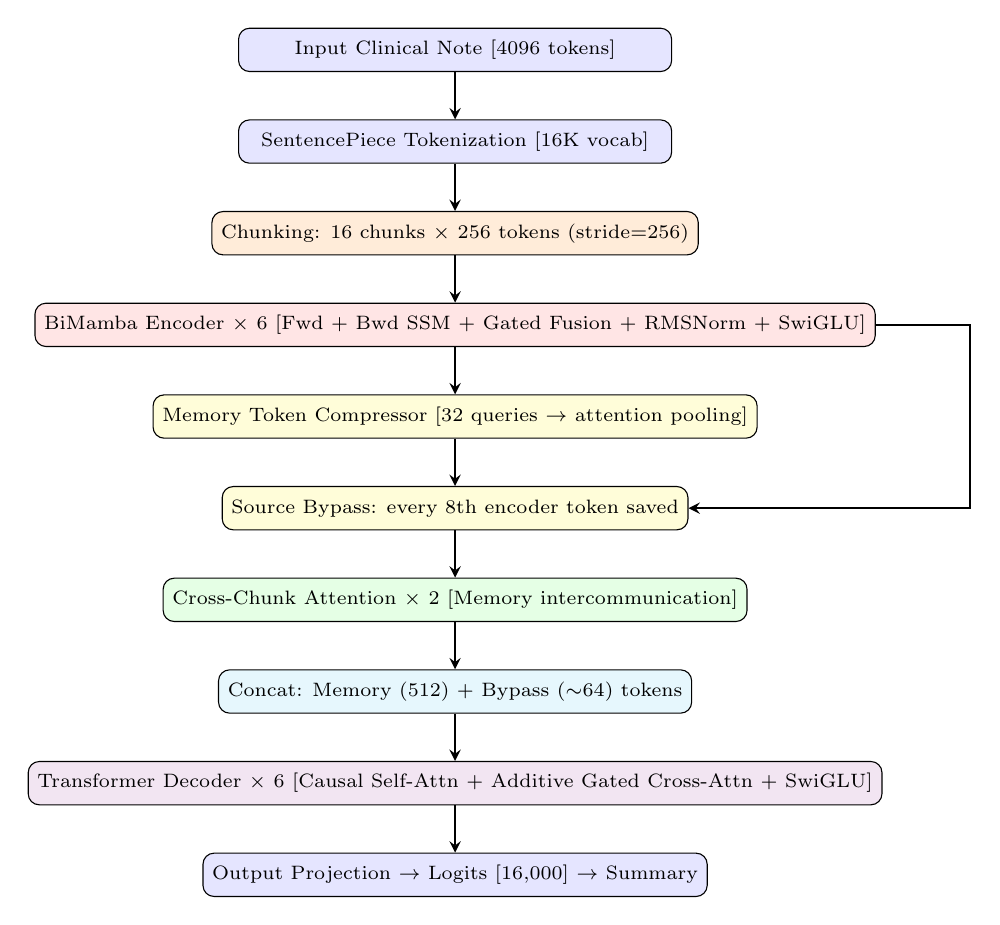
\begin{tikzpicture}[
      node distance=0.6cm,
      box/.style={draw, rounded corners, minimum width=5.5cm, minimum height=0.55cm, text centered, font=\scriptsize},
      arrow/.style={->, thick, >=stealth}
    ]
      \node[box, fill=blue!10] (input) {Input Clinical Note [4096 tokens]};
      \node[box, fill=blue!10, below=of input] (token) {SentencePiece Tokenization [16K vocab]};
      \node[box, fill=orange!15, below=of token] (chunk) {Chunking: 16 chunks $\times$ 256 tokens (stride=256)};
      \node[box, fill=red!10, below=of chunk] (bimamba) {BiMamba Encoder $\times$ 6 [Fwd + Bwd SSM + Gated Fusion + RMSNorm + SwiGLU]};
      \node[box, fill=yellow!15, below=of bimamba] (compress) {Memory Token Compressor [32 queries $\rightarrow$ attention pooling]};
      \node[box, fill=yellow!15, below=of compress] (bypass) {Source Bypass: every 8th encoder token saved};
      \node[box, fill=green!10, below=of bypass] (cross) {Cross-Chunk Attention $\times$ 2 [Memory intercommunication]};
      \node[box, fill=cyan!10, below=of cross] (concat) {Concat: Memory (512) + Bypass ($\sim$64) tokens};
      \node[box, fill=violet!10, below=of concat] (decoder) {Transformer Decoder $\times$ 6 [Causal Self-Attn + Additive Gated Cross-Attn + SwiGLU]};
      \node[box, fill=blue!10, below=of decoder] (output) {Output Projection $\rightarrow$ Logits [16,000] $\rightarrow$ Summary};

      \draw[arrow] (input) -- (token);
      \draw[arrow] (token) -- (chunk);
      \draw[arrow] (chunk) -- (bimamba);
      \draw[arrow] (bimamba) -- (compress);
      \draw[arrow] (bimamba.east) -- ++(1.2,0) |- (bypass.east);
      \draw[arrow] (compress) -- (bypass);
      \draw[arrow] (bypass) -- (cross);
      \draw[arrow] (cross) -- (concat);
      \draw[arrow] (concat) -- (decoder);
      \draw[arrow] (decoder) -- (output);
    \end{tikzpicture}
  \end{center}
\end{frame}

% ============================================================
% SECTION 6: RESULTS & DISCUSSION
% ============================================================
\section{Results and Discussion}

\begin{frame}{ROUGE Score Comparison}
  \begin{center}
    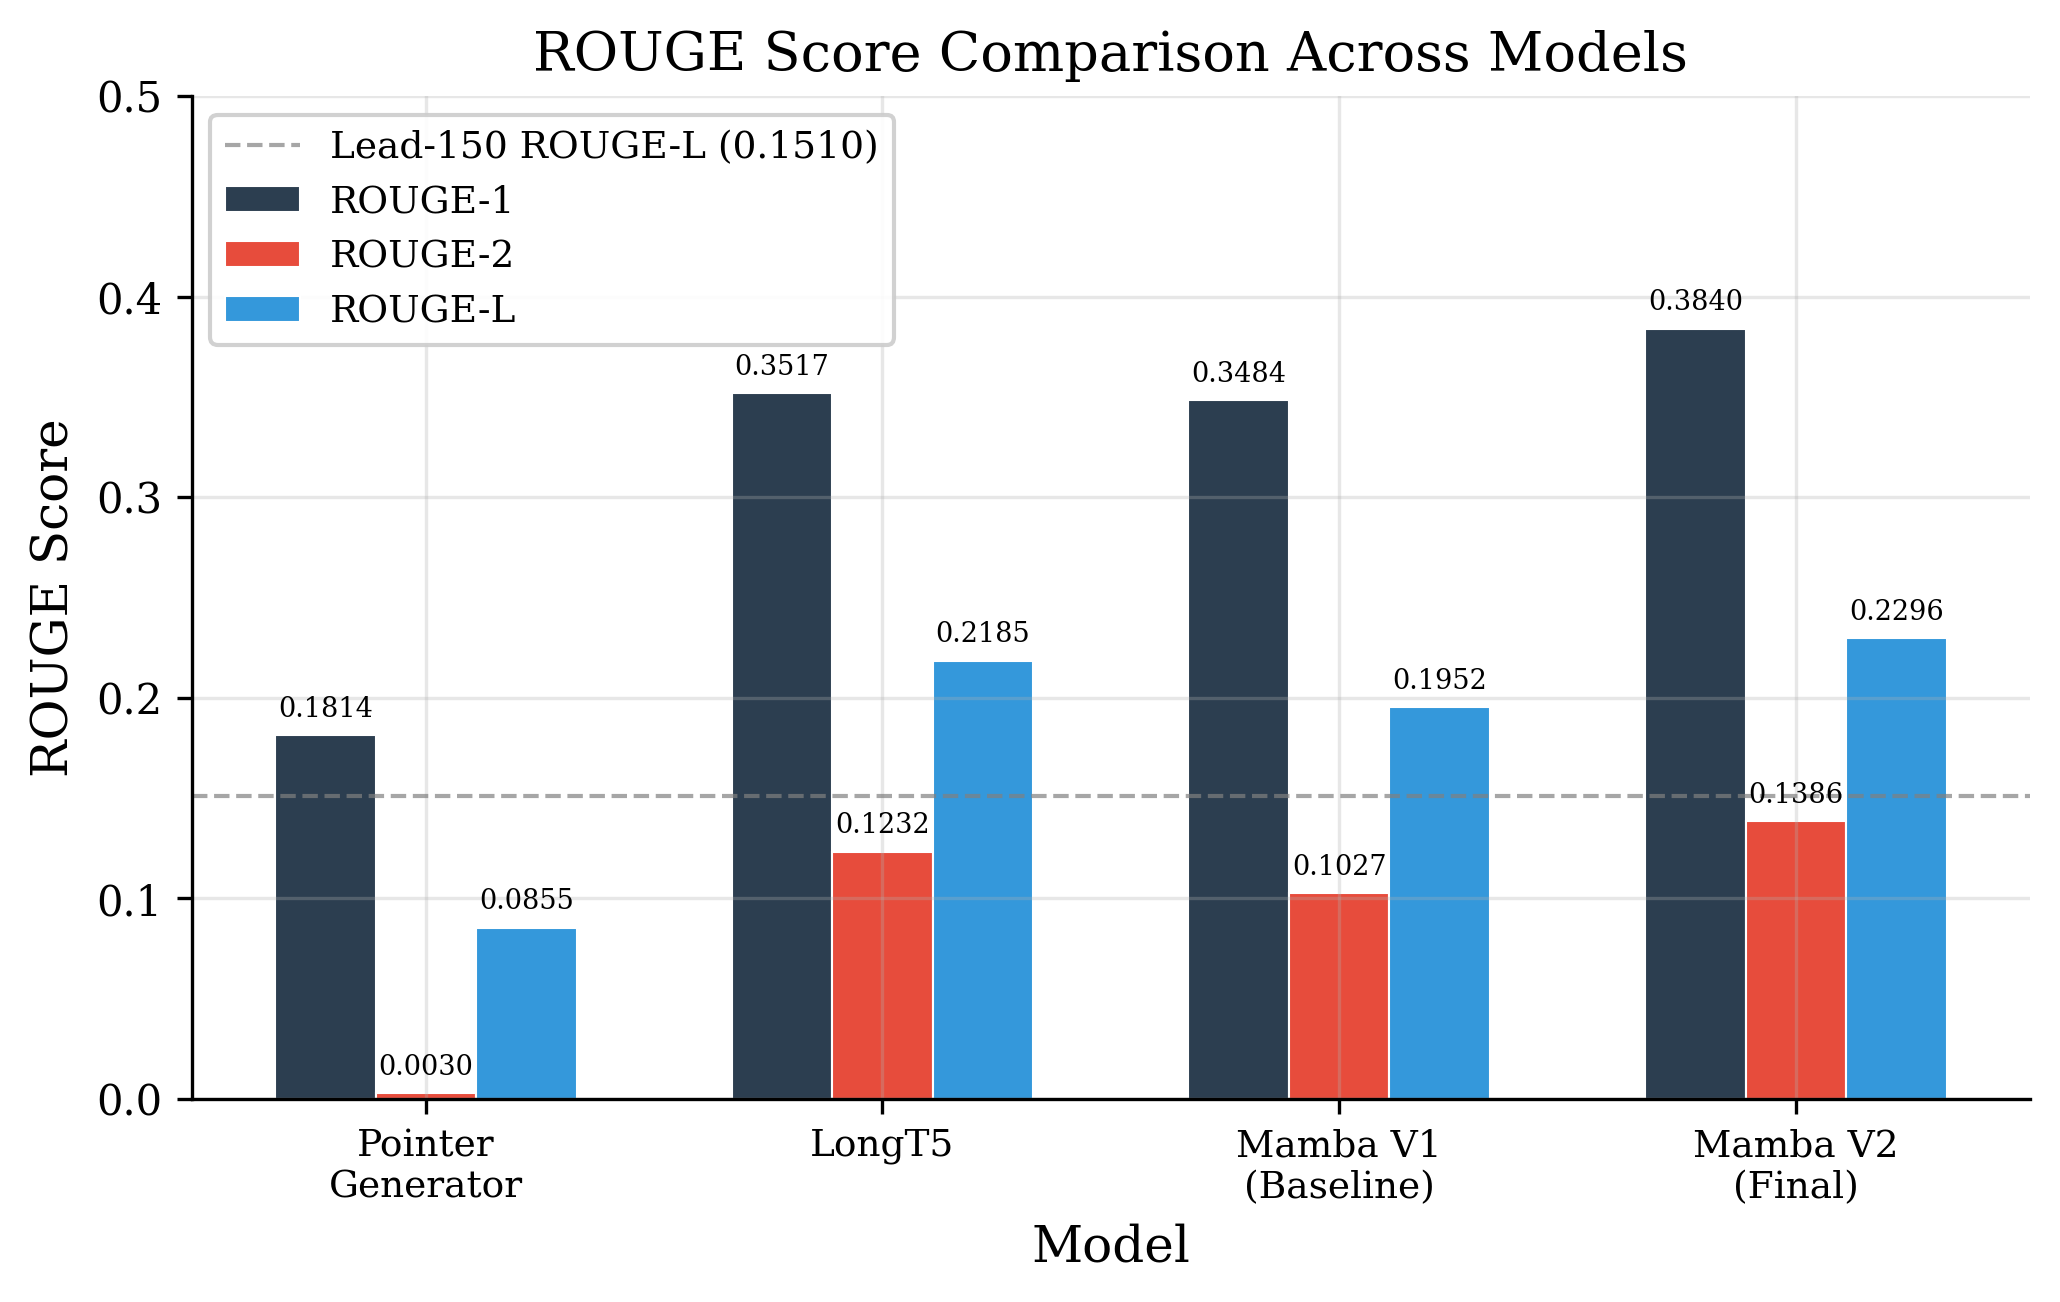
\includegraphics[width=0.7\textwidth]{figures/rouge_comparison.png}
  \end{center}
  \vspace{-0.3cm}
  {\small Mamba V2 (best at step 130K): R-1=0.3840, R-2=0.1386, R-L=0.2296 --- surpassing Lead-150 by 52.1\% on ROUGE-L.}
\end{frame}

\begin{frame}{Why ROUGE Metrics? Evaluation Strategy Rationale}
  \footnotesize
  \begin{columns}[T]
    \begin{column}{0.48\textwidth}
      \textbf{Metric Comparison for Summarization:}
      \begin{table}
        \centering
        \scriptsize
        \renewcommand{\arraystretch}{1.15}
        \begin{tabular}{l|cccc}
          \toprule
          & \textbf{ROUGE} & \textbf{BLEU} & \textbf{METEOR} & \textbf{BERTSc.} \\
          \midrule
          Task Fit & \textcolor{darkgreen}{\textbf{Summ.}} & MT & MT & Any \\
          Focus & Recall & Prec. & Both & Sem. \\
          Speed & \textcolor{darkgreen}{\textbf{Fast}} & Fast & Med. & Slow \\
          Standard & \textcolor{darkgreen}{\textbf{Yes}} & No & No & New \\
          GPU? & No & No & No & \textcolor{darkred}{Yes} \\
          \bottomrule
        \end{tabular}
      \end{table}
      \vspace{-0.1cm}
      {\scriptsize MT = Machine Translation primary use.}
    \end{column}
    \begin{column}{0.48\textwidth}
      \textbf{Why ROUGE over BLEU?}
      \begin{itemize}\setlength{\itemsep}{0pt}
        \item ROUGE is \textbf{recall-oriented} --- measures how much of the reference appears in the summary (critical for clinical completeness)
        \item BLEU is \textbf{precision-oriented} --- designed for MT, penalizes short outputs rather than missing content
        \item ROUGE-1/2/L is the \textbf{de-facto standard} for summarization (ACL, NAACL benchmarks)
      \end{itemize}

      \vspace{0.1cm}
      \textbf{Why NOT BERTScore alone?}
      \begin{itemize}\setlength{\itemsep}{0pt}
        \item Requires GPU inference --- slow for 270K samples
        \item Less interpretable than n-gram overlap
        \item We propose it for \textbf{future clinical eval} (Gate 4)
      \end{itemize}
    \end{column}
  \end{columns}
\end{frame}

\begin{frame}{Why Beam Search \& Cross-Entropy Loss?}
  \footnotesize
  \begin{columns}[T]
    \begin{column}{0.48\textwidth}
      \textbf{Decoding Strategy Comparison:}
      \begin{table}
        \centering
        \scriptsize
        \renewcommand{\arraystretch}{1.15}
        \begin{tabular}{l|ccc}
          \toprule
          \textbf{Method} & \textbf{Greedy} & \textbf{Beam} & \textbf{Nucleus} \\
          \midrule
          Quality & Low & \textcolor{darkgreen}{\textbf{High}} & Variable \\
          Determin. & Yes & \textcolor{darkgreen}{\textbf{Yes}} & No \\
          Diversity & None & Moderate & High \\
          Clinical? & Unsafe & \textcolor{darkgreen}{\textbf{Safe}} & Risky \\
          \bottomrule
        \end{tabular}
      \end{table}
      \vspace{-0.1cm}
      \textbf{Why Beam Search (width=4)?}
      \begin{itemize}\setlength{\itemsep}{0pt}
        \item \textbf{Deterministic:} Clinical summaries must be reproducible
        \item \textbf{Greedy} misses global optima --- local decisions only
        \item \textbf{Nucleus/Top-k sampling} --- randomness is unacceptable for medical documents
        \item Width=4 balances quality vs.\ compute on 8~GB GPU
      \end{itemize}
    \end{column}
    \begin{column}{0.48\textwidth}
      \textbf{Why Cross-Entropy Loss (not others)?}
      \begin{itemize}\setlength{\itemsep}{0pt}
        \item \textbf{Standard} for sequence-to-sequence text generation
        \item \textbf{Focal Loss:} Designed for class imbalance (detection), not seq2seq
        \item \textbf{Label Smoothing:} Omitted intentionally --- clinical terms need sharp probability peaks, not soft distributions
        \item \textbf{Contrastive Loss:} For representation learning, not autoregressive generation
      \end{itemize}

      \vspace{0.1cm}
      \textbf{Why N-gram Blocking ($n{=}3$)?}
      \begin{itemize}\setlength{\itemsep}{0pt}
        \item Prevents repetitive phrases (common in seq2seq)
        \item $n{=}3$ blocks repeated trigrams while allowing natural medical repetition (``blood pressure'')
        \item Combined with length penalty (0.8) to discourage overly short outputs
      \end{itemize}
    \end{column}
  \end{columns}
\end{frame}

\begin{frame}{Why Mamba V2 Wins: Explaining the Results}
  \small
  \begin{columns}[T]
    \begin{column}{0.48\textwidth}
      \textbf{ROUGE-1 (Unigram): 0.3840}
      \begin{itemize}\setlength{\itemsep}{0pt}
        \item \textbf{Source bypass}: direct access to encoder tokens
        \item \textbf{No label smoothing}: sharper vocabulary predictions
        \item 150K steps $\rightarrow$ thorough clinical vocab learning
      \end{itemize}

      \vspace{0.1cm}
      \textbf{ROUGE-2 (Bigram): 0.1386}
      \begin{itemize}\setlength{\itemsep}{0pt}
        \item \textbf{4,520\%} over PG (0.003 $\rightarrow$ 0.1386): coherent \emph{phrases}
        \item \textbf{SwiGLU}: better sequential token prediction
        \item \textbf{Additive gating}: bigram patterns not suppressed
      \end{itemize}
    \end{column}
    \begin{column}{0.48\textwidth}
      \textbf{ROUGE-L (LCS): 0.2296 --- +168.5\% vs PG}
      \begin{itemize}\setlength{\itemsep}{0pt}
        \item ROUGE-L measures structural coherence --- does the summary follow the source's logical flow?
        \item \textbf{BiMamba}: rich encodings respecting clinical narrative order
        \item \textbf{Memory + bypass}: abstract summary + exact details
        \item \textbf{Additive gate fix}: single biggest contributor (without it, 98.4\% signal lost)
      \end{itemize}

      \vspace{0.1cm}
      \textbf{vs.\ Lead-150 Baseline:}
      \begin{itemize}\setlength{\itemsep}{0pt}
        \item Lead-150 R-L = 0.1510; V2 = 0.2296 (\textcolor{darkgreen}{+52.1\%})
        \item Model generates \emph{abstractions}, not just copying
      \end{itemize}
    \end{column}
  \end{columns}
\end{frame}

\begin{frame}{ROUGE-L Progression Across Models}
  \begin{columns}[T]
    \begin{column}{0.55\textwidth}
      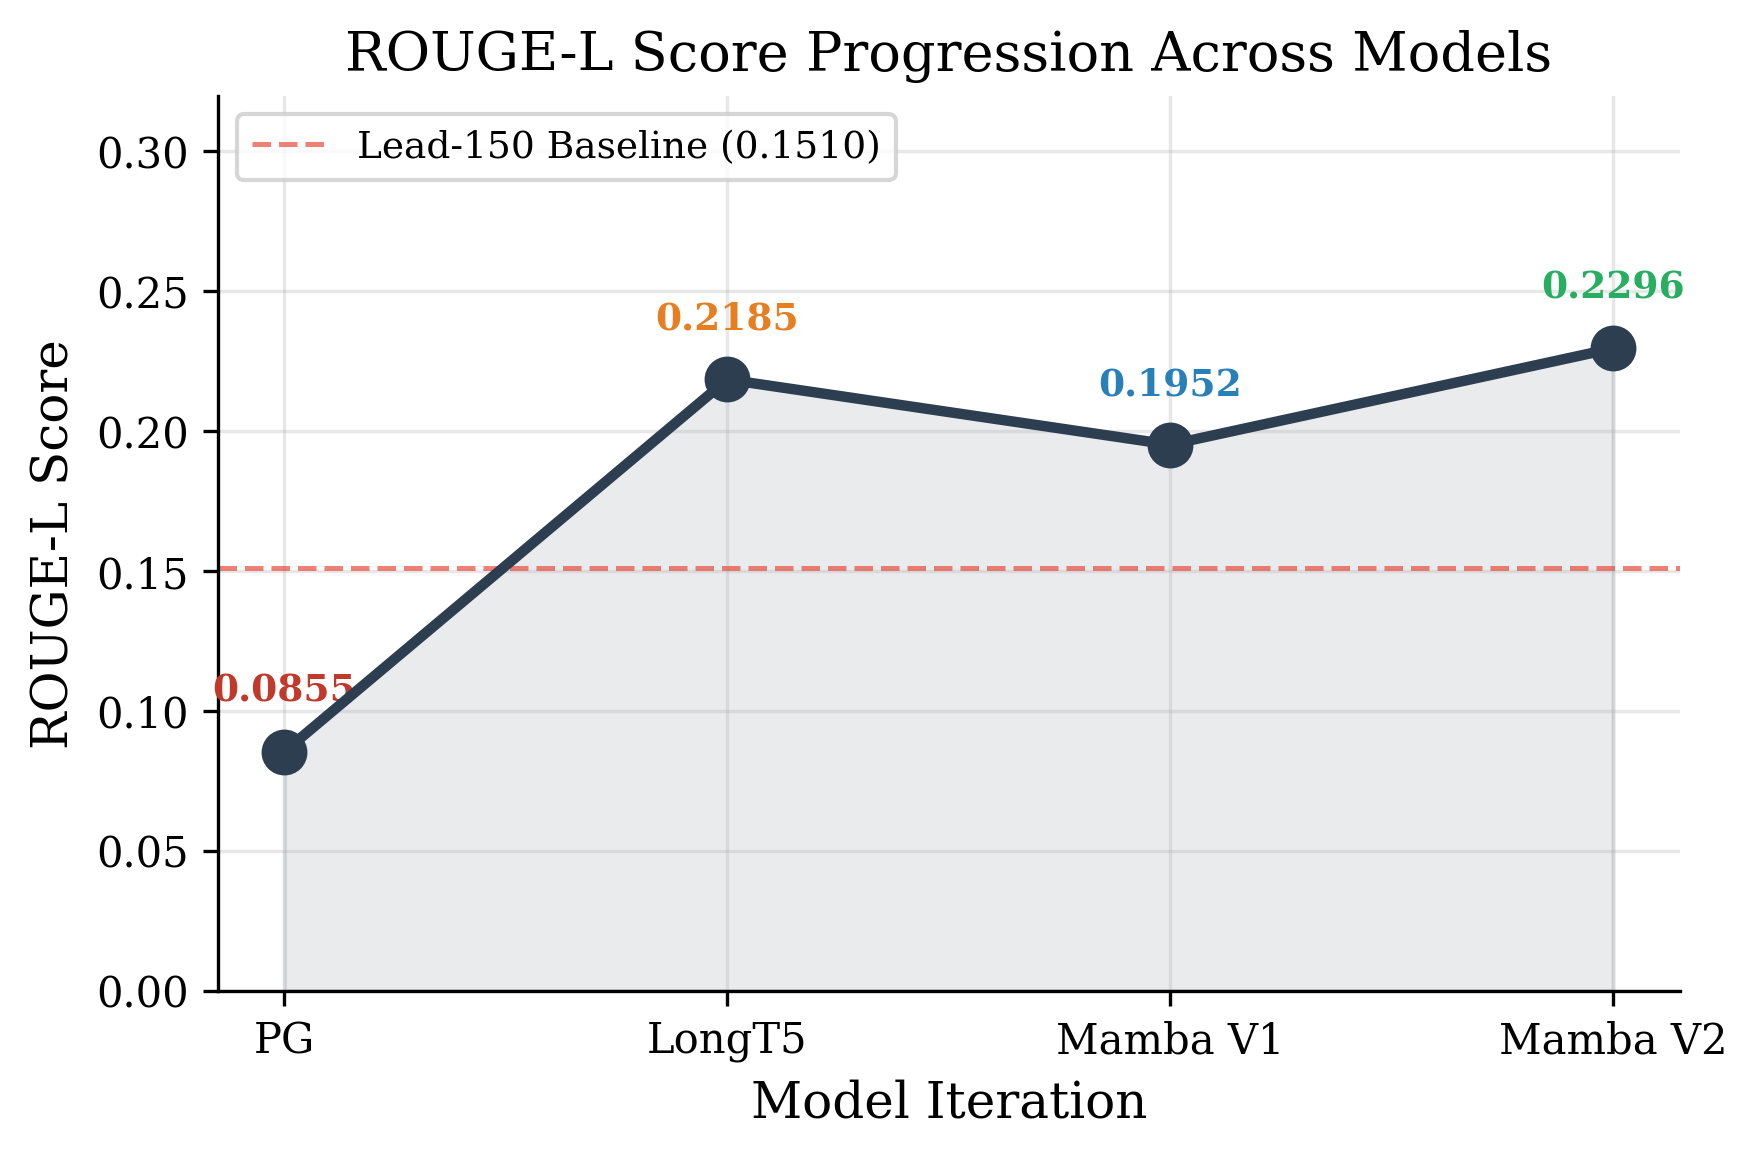
\includegraphics[width=\textwidth]{figures/rougeL_progression.png}
    \end{column}
    \begin{column}{0.42\textwidth}
      \textbf{Progressive Improvement:}
      \begin{itemize}
        \item PG $\rightarrow$ LongT5: \textcolor{darkgreen}{+155.6\%}\\
          {\scriptsize (4096-token input, streaming)}
        \item LongT5 $\rightarrow$ Mamba V1: \textcolor{amber}{$-$10.7\%}\\
          {\scriptsize (SSM encoder, but cross-attn bug)}
        \item V1 $\rightarrow$ V2: \textcolor{darkgreen}{+17.6\%}\\
          {\scriptsize (Gate fix, SwiGLU, bypass, 150K steps)}
      \end{itemize}

      \vspace{0.2cm}
      \textbf{Total improvement:}\\
      \textcolor{darkgreen}{\textbf{+168.5\%}} from Pointer-Generator to Mamba V2 (0.0855 $\rightarrow$ 0.2296).
    \end{column}
  \end{columns}
\end{frame}

\begin{frame}{Training Loss Comparison}
  \begin{columns}[T]
    \begin{column}{0.52\textwidth}
      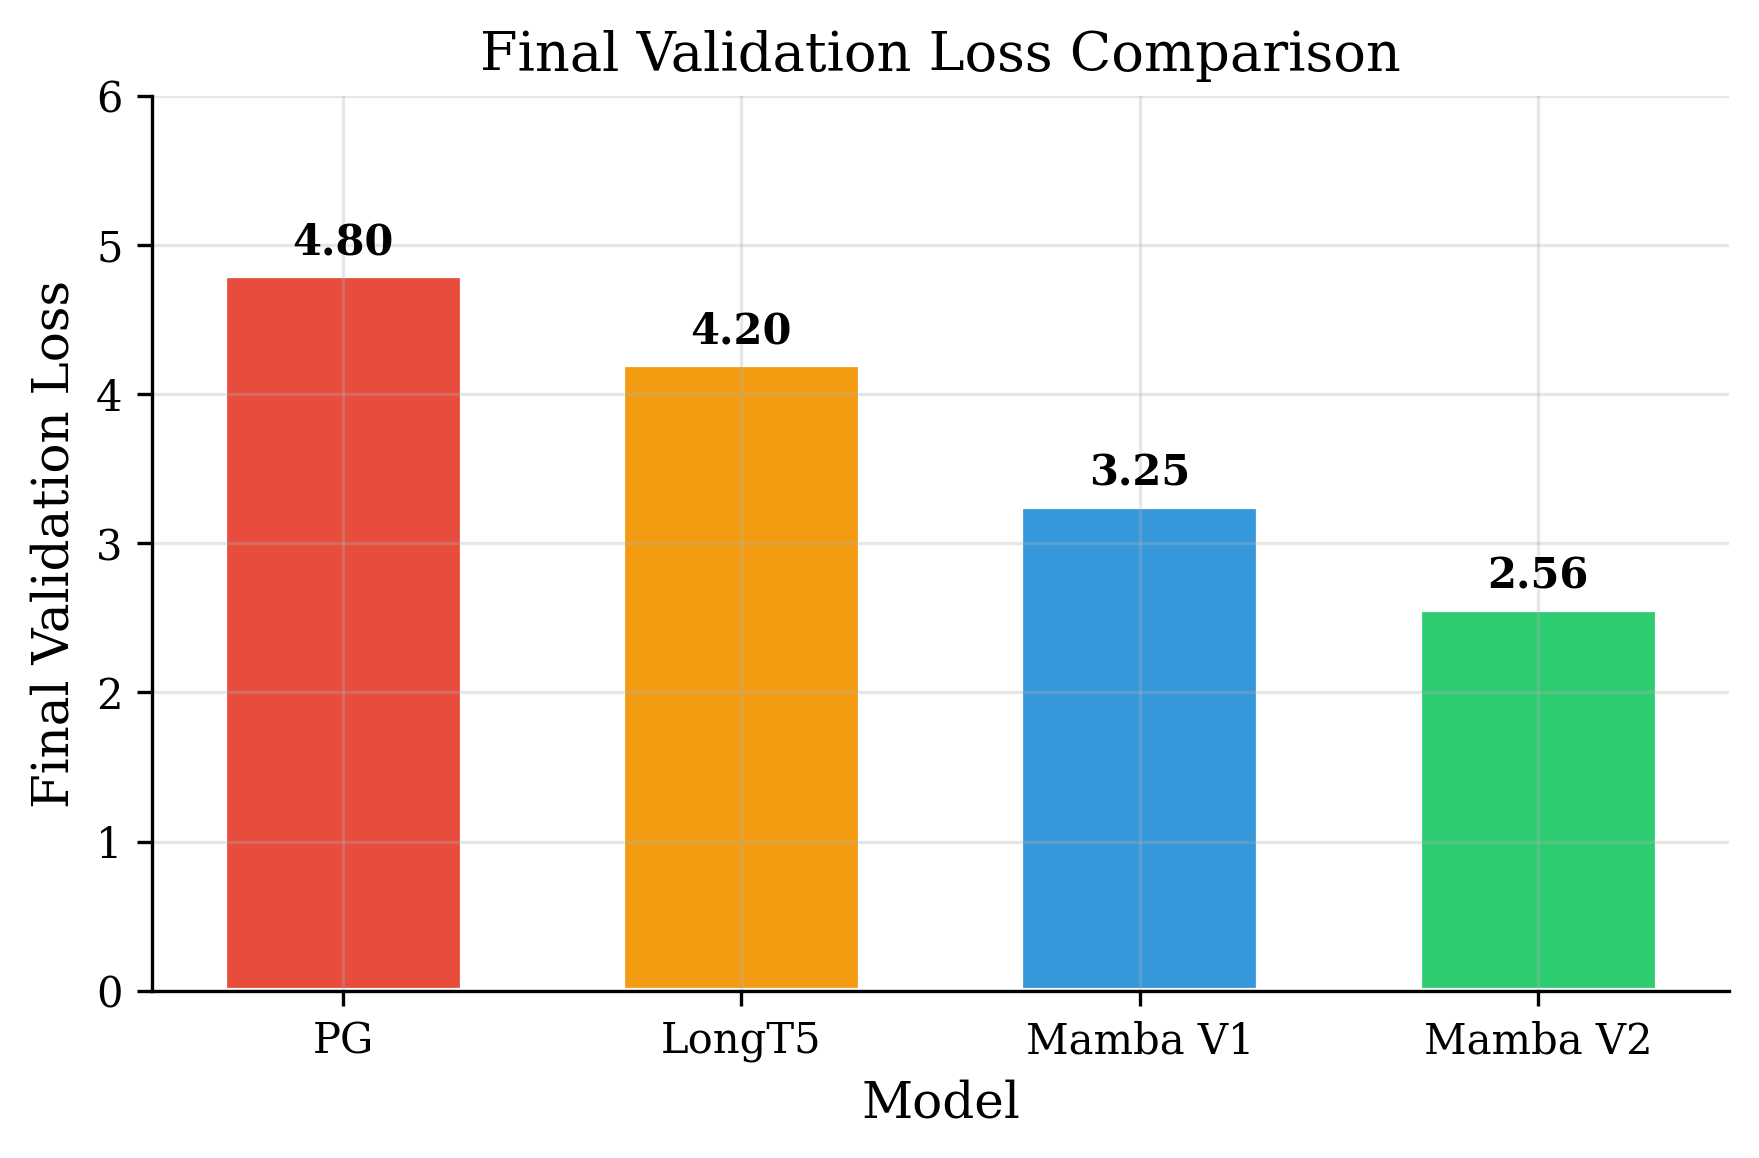
\includegraphics[width=\textwidth]{figures/training_loss_comparison.png}
    \end{column}
    \begin{column}{0.45\textwidth}
      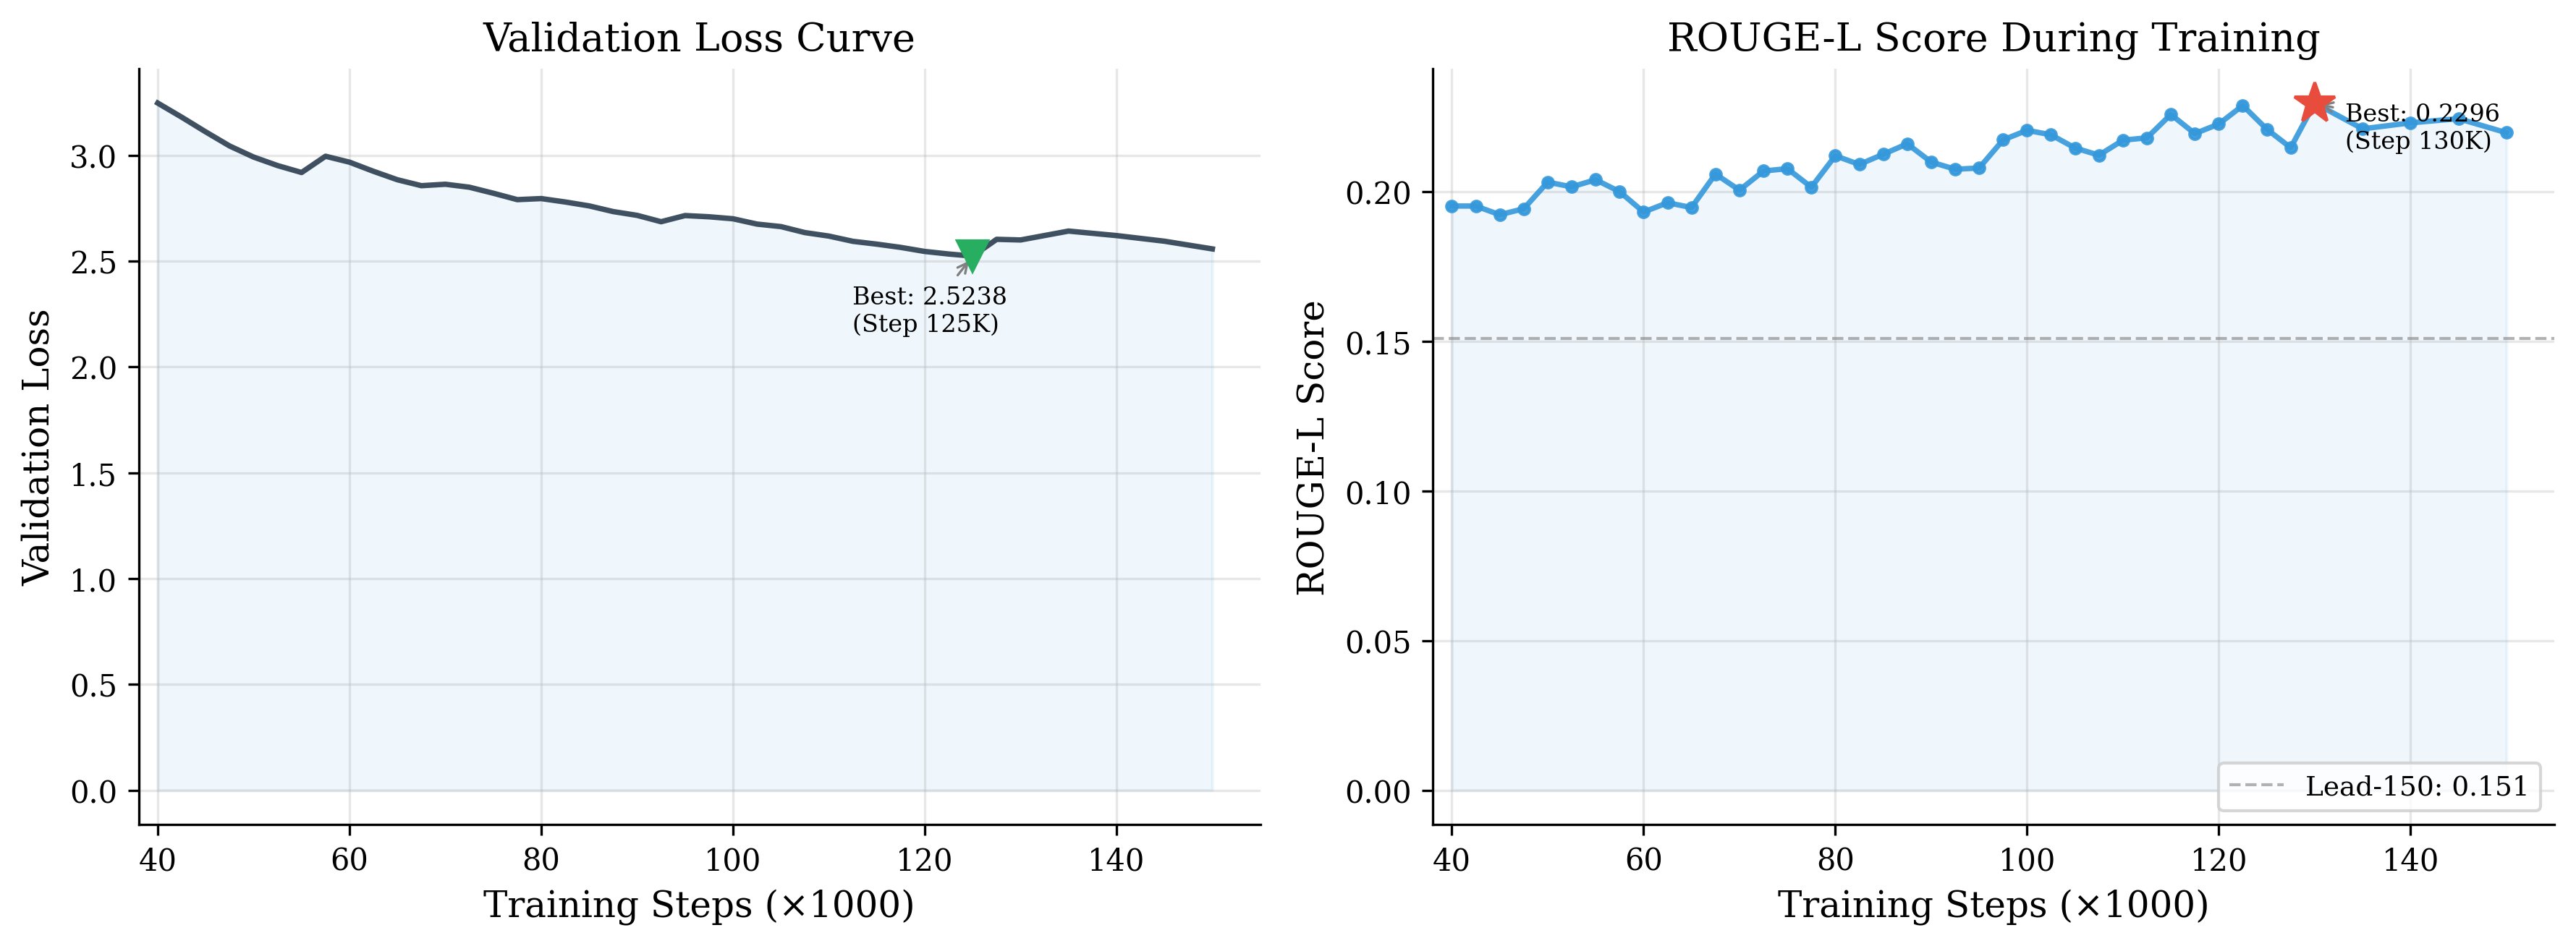
\includegraphics[width=\textwidth]{figures/mamba_training_curve.png}
    \end{column}
  \end{columns}

  \vspace{0.2cm}
  {\small Mamba V2 training \textbf{completed all 150,000 steps}. Validation loss decreased from 3.25 $\rightarrow$ 2.56 (21.2\% improvement). Best ROUGE-L occurred at step 130K (0.2296), with the model showing continued convergence.}
\end{frame}

\begin{frame}{Mamba V2: Complete Training Trajectory}
  \begin{columns}[T]
    \begin{column}{0.55\textwidth}
      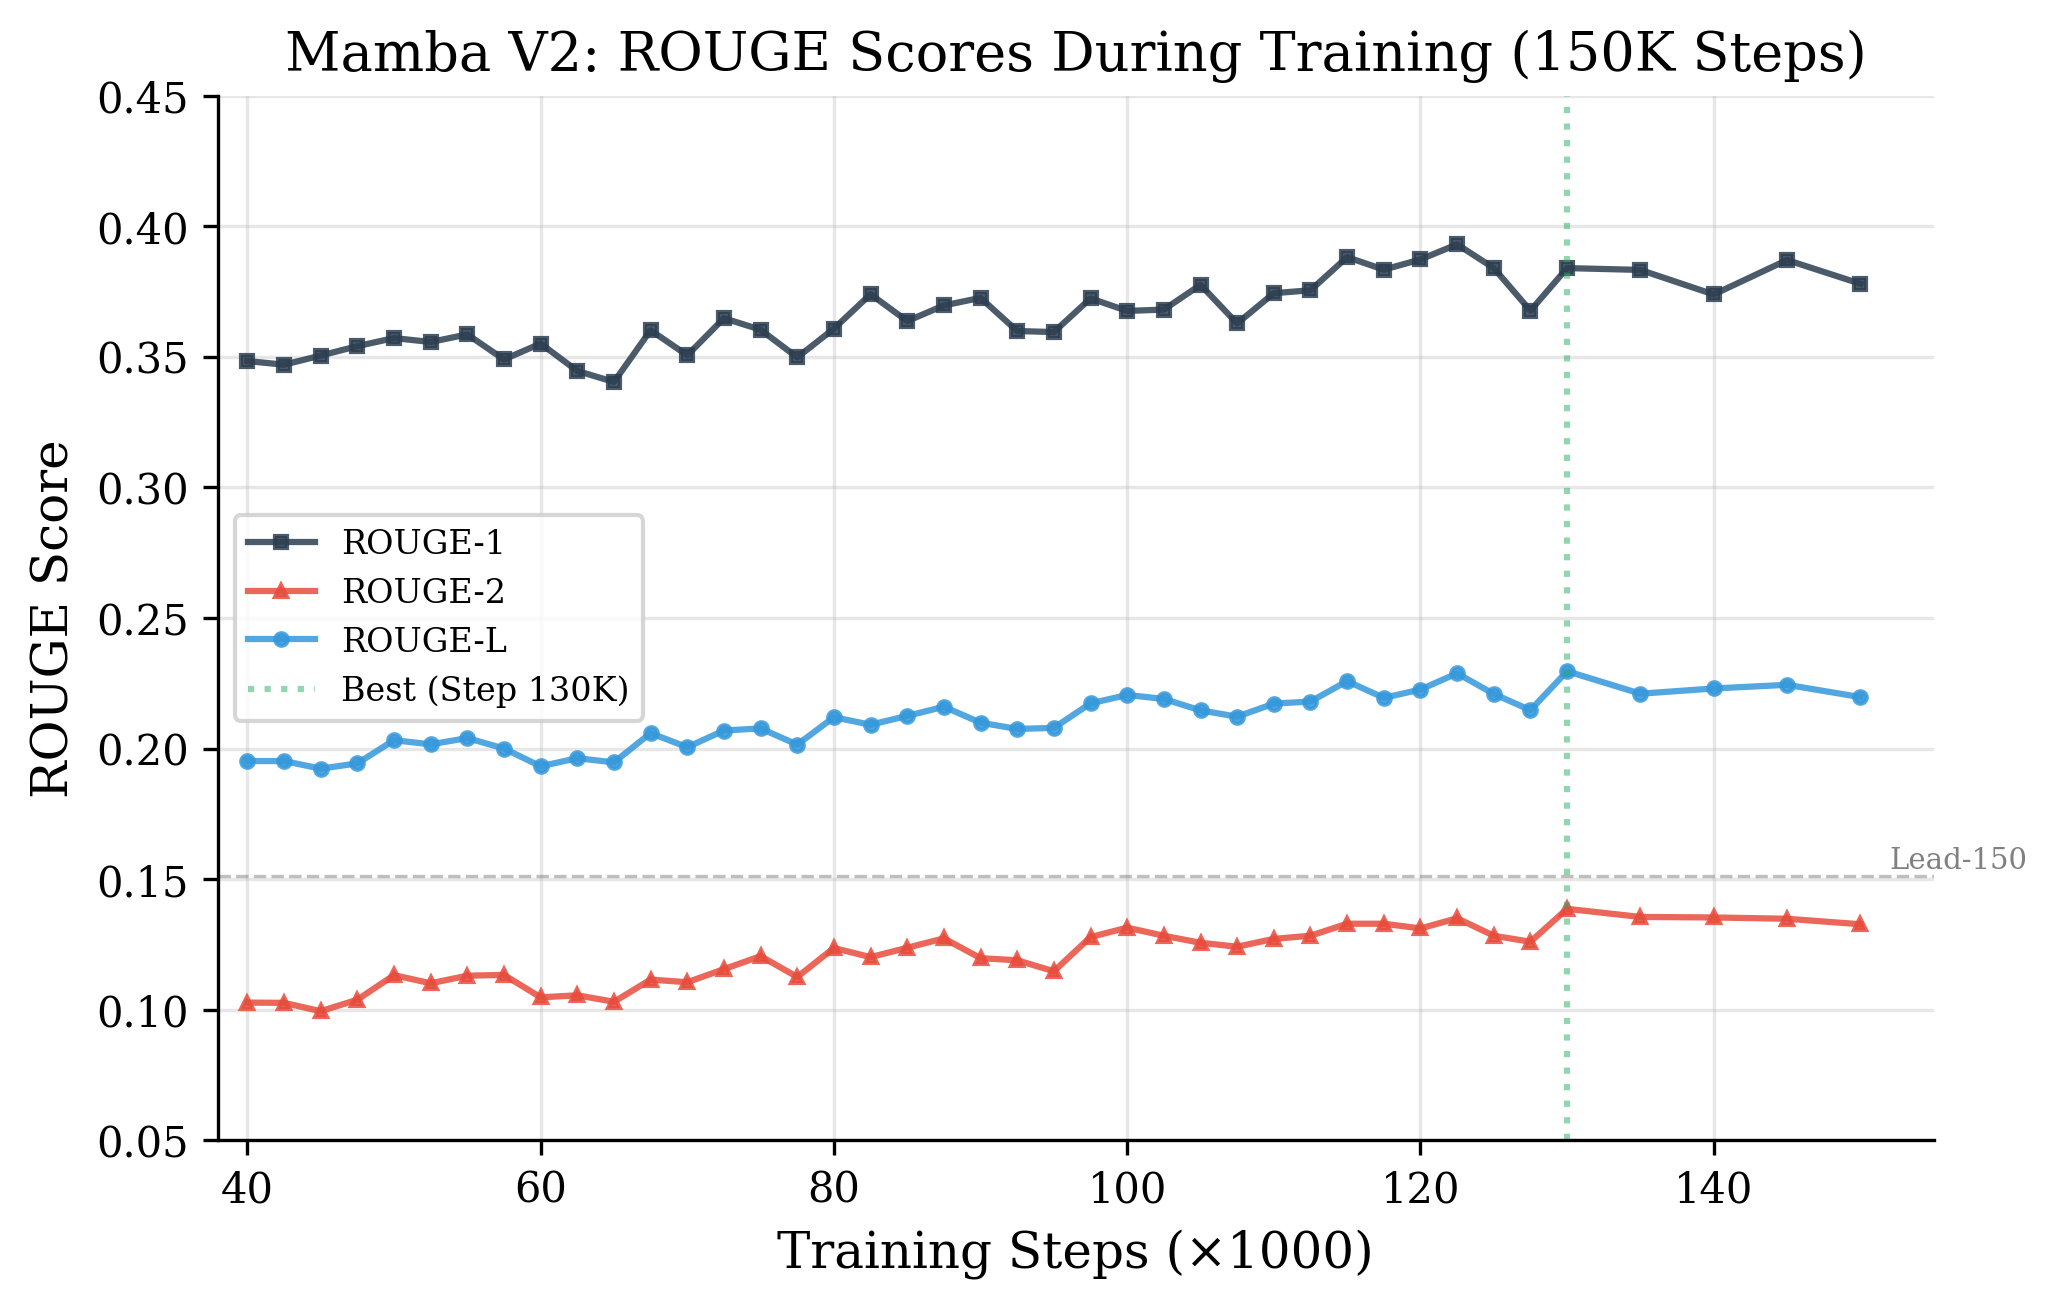
\includegraphics[width=\textwidth]{figures/v2_rouge_training.png}
    \end{column}
    \begin{column}{0.42\textwidth}
      \textbf{43 Evaluation Points (40K--150K):}
      \begin{itemize}
        \item ROUGE-1: 0.3484 $\rightarrow$ 0.3840 (peak)
        \item ROUGE-2: 0.1027 $\rightarrow$ 0.1386 (peak)
        \item ROUGE-L: 0.1952 $\rightarrow$ 0.2296 (peak)
        \item Best model: \textbf{Step 130K}
        \item Final model (150K): R-L = 0.2197
      \end{itemize}

      \vspace{0.2cm}
      \textbf{Key Observations:}
      \begin{itemize}
        \item Steady improvement with occasional fluctuations (normal for cosine warm restarts)
        \item Best ROUGE-L at 130K, slight decline afterward --- \textbf{early stopping captured best model}
        \item All 3 ROUGE metrics peaked near 130K, confirming convergence
      \end{itemize}
    \end{column}
  \end{columns}
\end{frame}

\begin{frame}{ROUGE-2 Improvement \& Percentage Gains}
  \begin{columns}[T]
    \begin{column}{0.48\textwidth}
      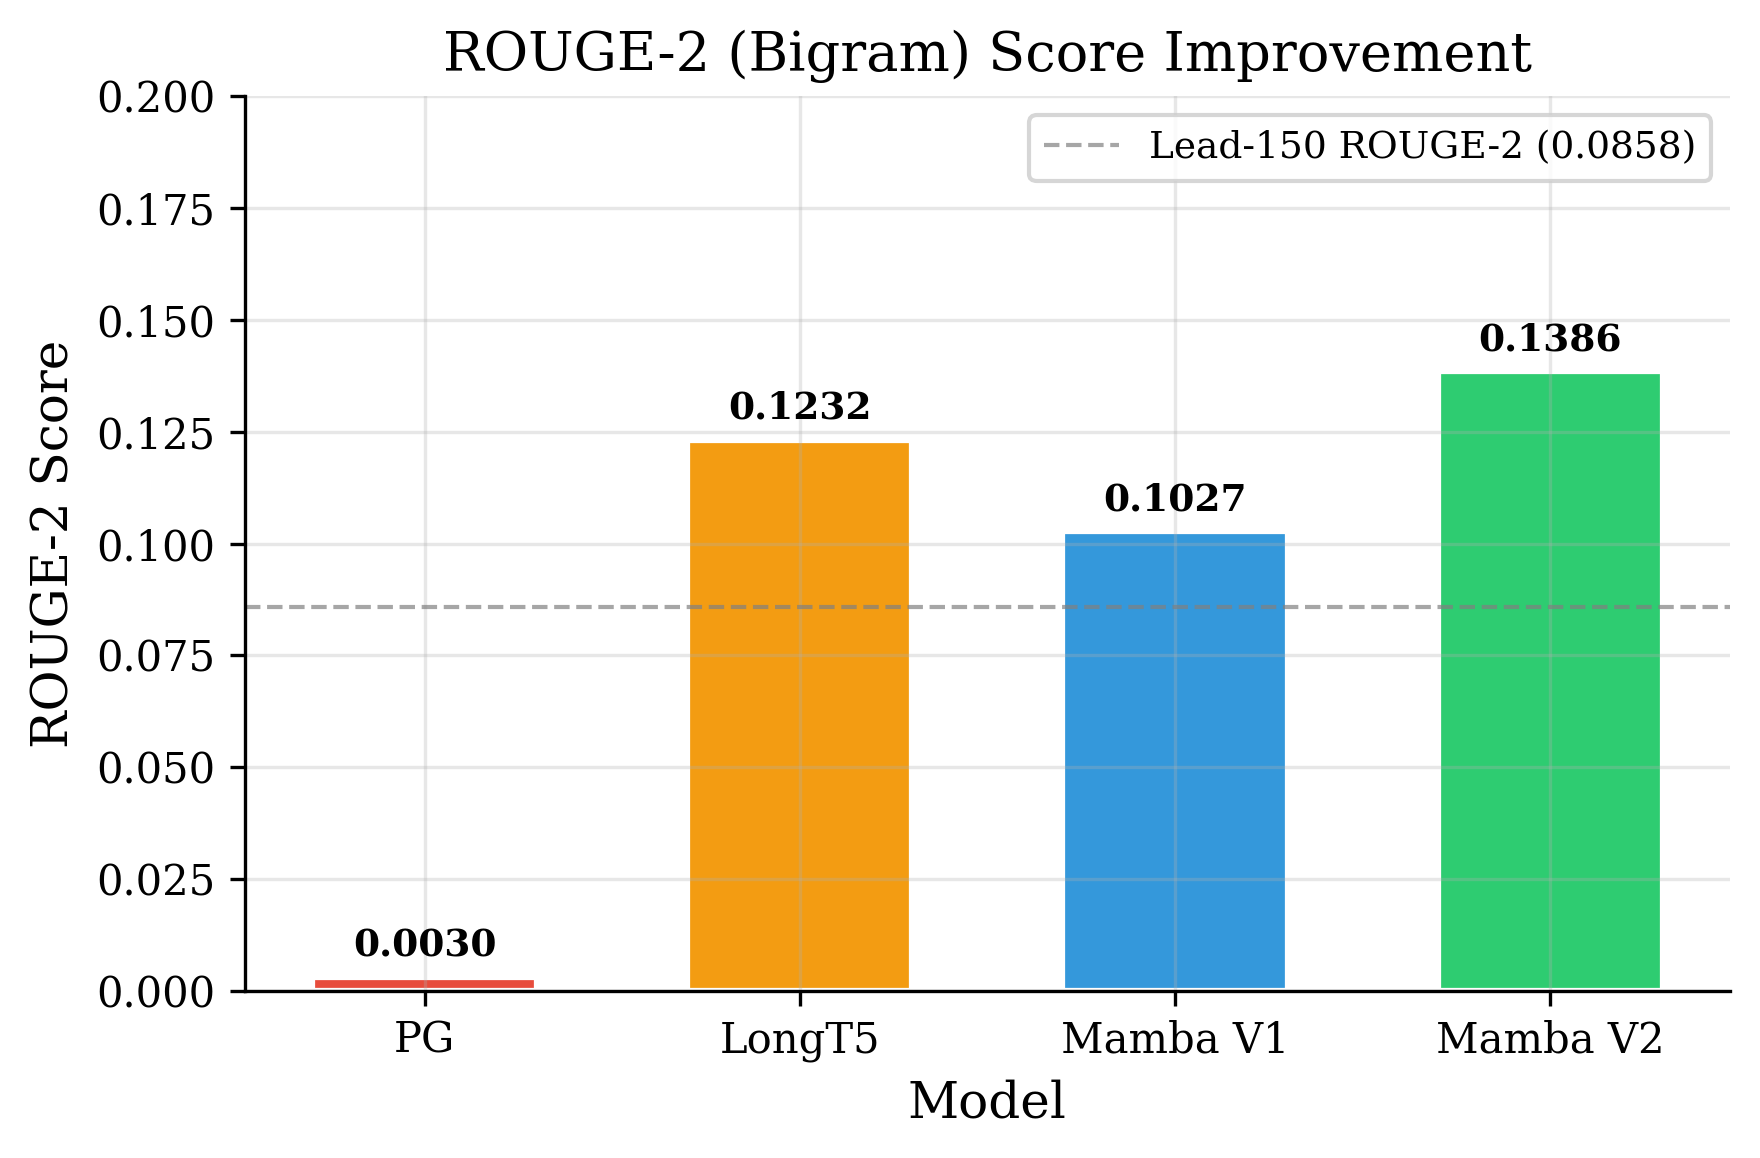
\includegraphics[width=\textwidth]{figures/rouge2_improvement.png}\\
      {\scriptsize ROUGE-2 (bigram): from near-zero (0.003) to 0.1386 --- model now generates coherent multi-word clinical phrases.}
    \end{column}
    \begin{column}{0.48\textwidth}
      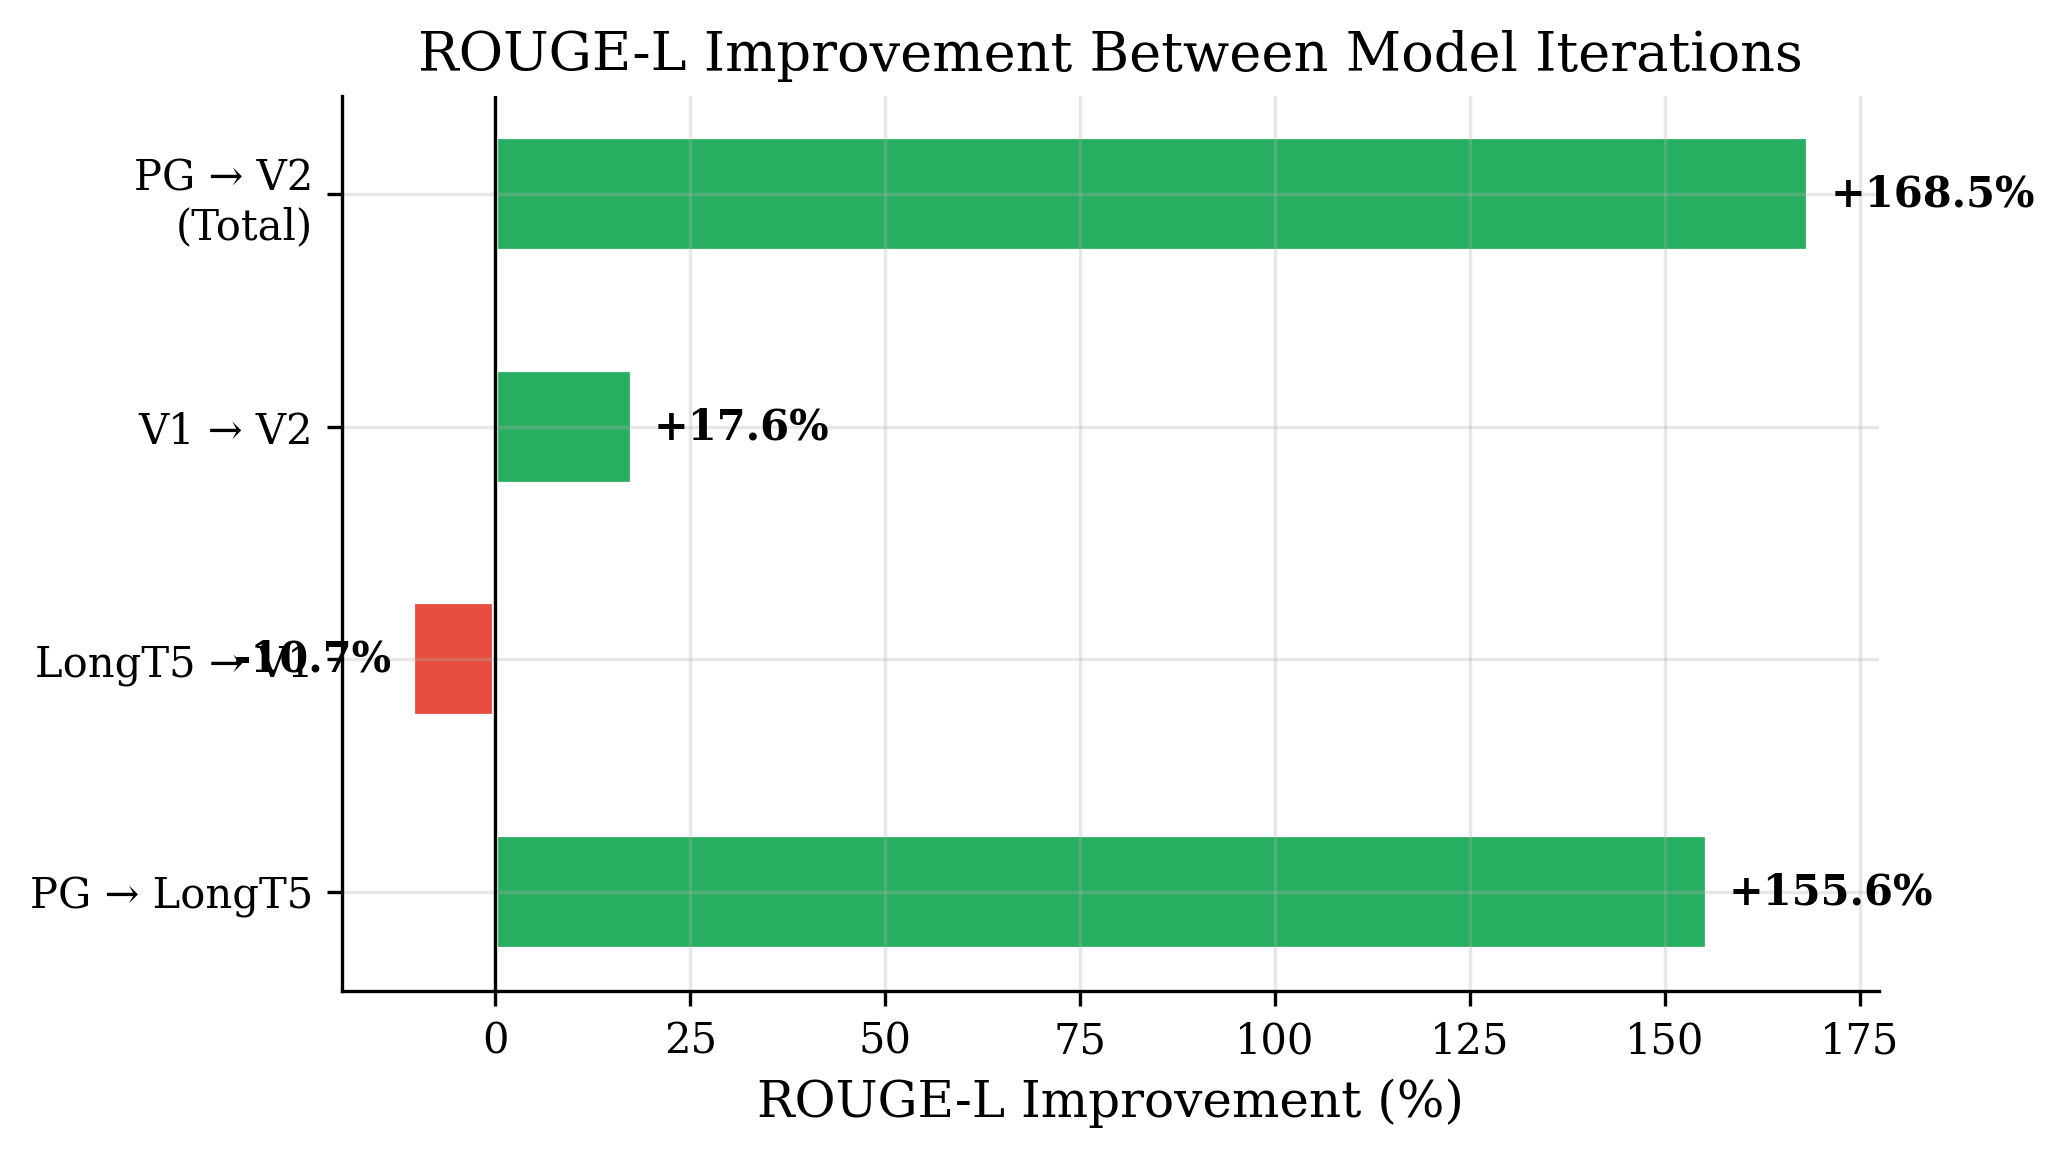
\includegraphics[width=\textwidth]{figures/improvement_pct.png}\\
      {\scriptsize Note: LongT5 $\rightarrow$ V1 shows a \textbf{decrease} because Mamba V1 had the cross-attention gating bug. V2 fixed this and exceeded LongT5.}
    \end{column}
  \end{columns}
\end{frame}

\begin{frame}{Model Complexity Analysis}
  \begin{columns}[T]
    \begin{column}{0.48\textwidth}
      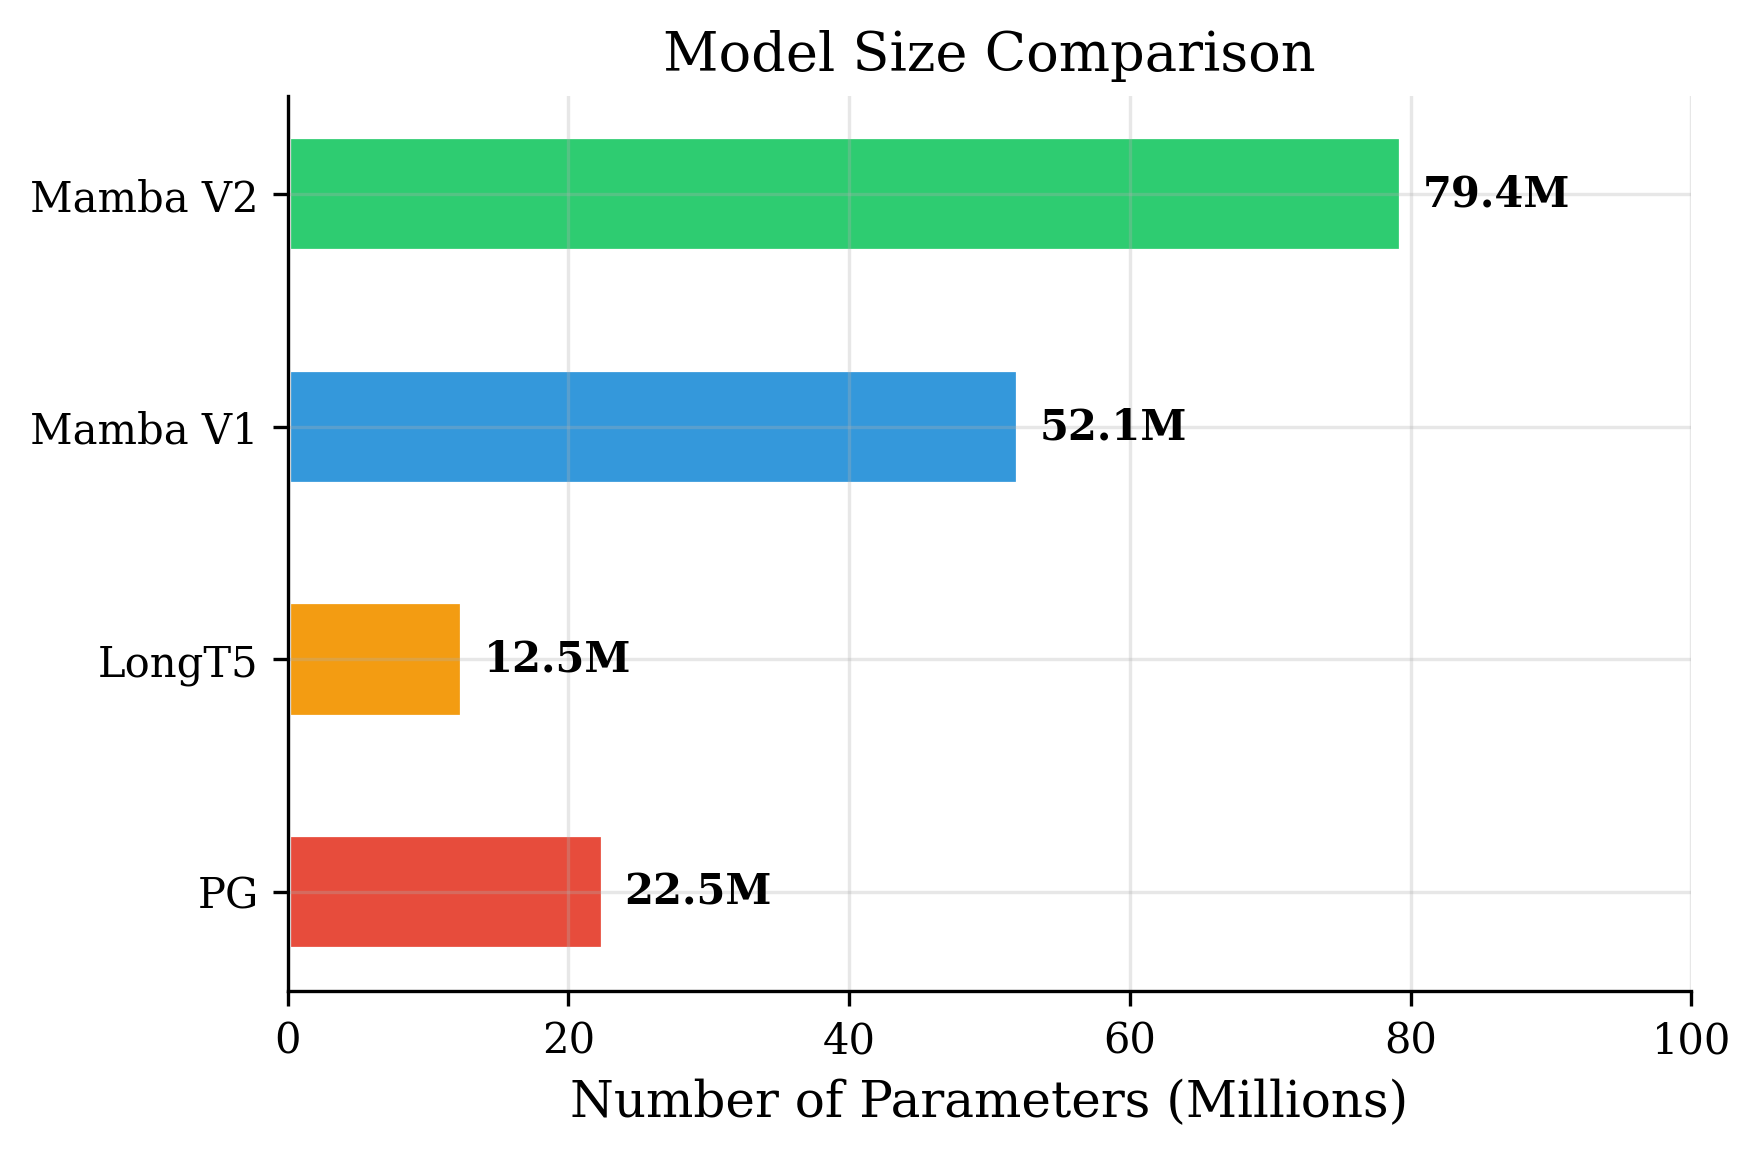
\includegraphics[width=\textwidth]{figures/model_parameters.png}
    \end{column}
    \begin{column}{0.48\textwidth}
      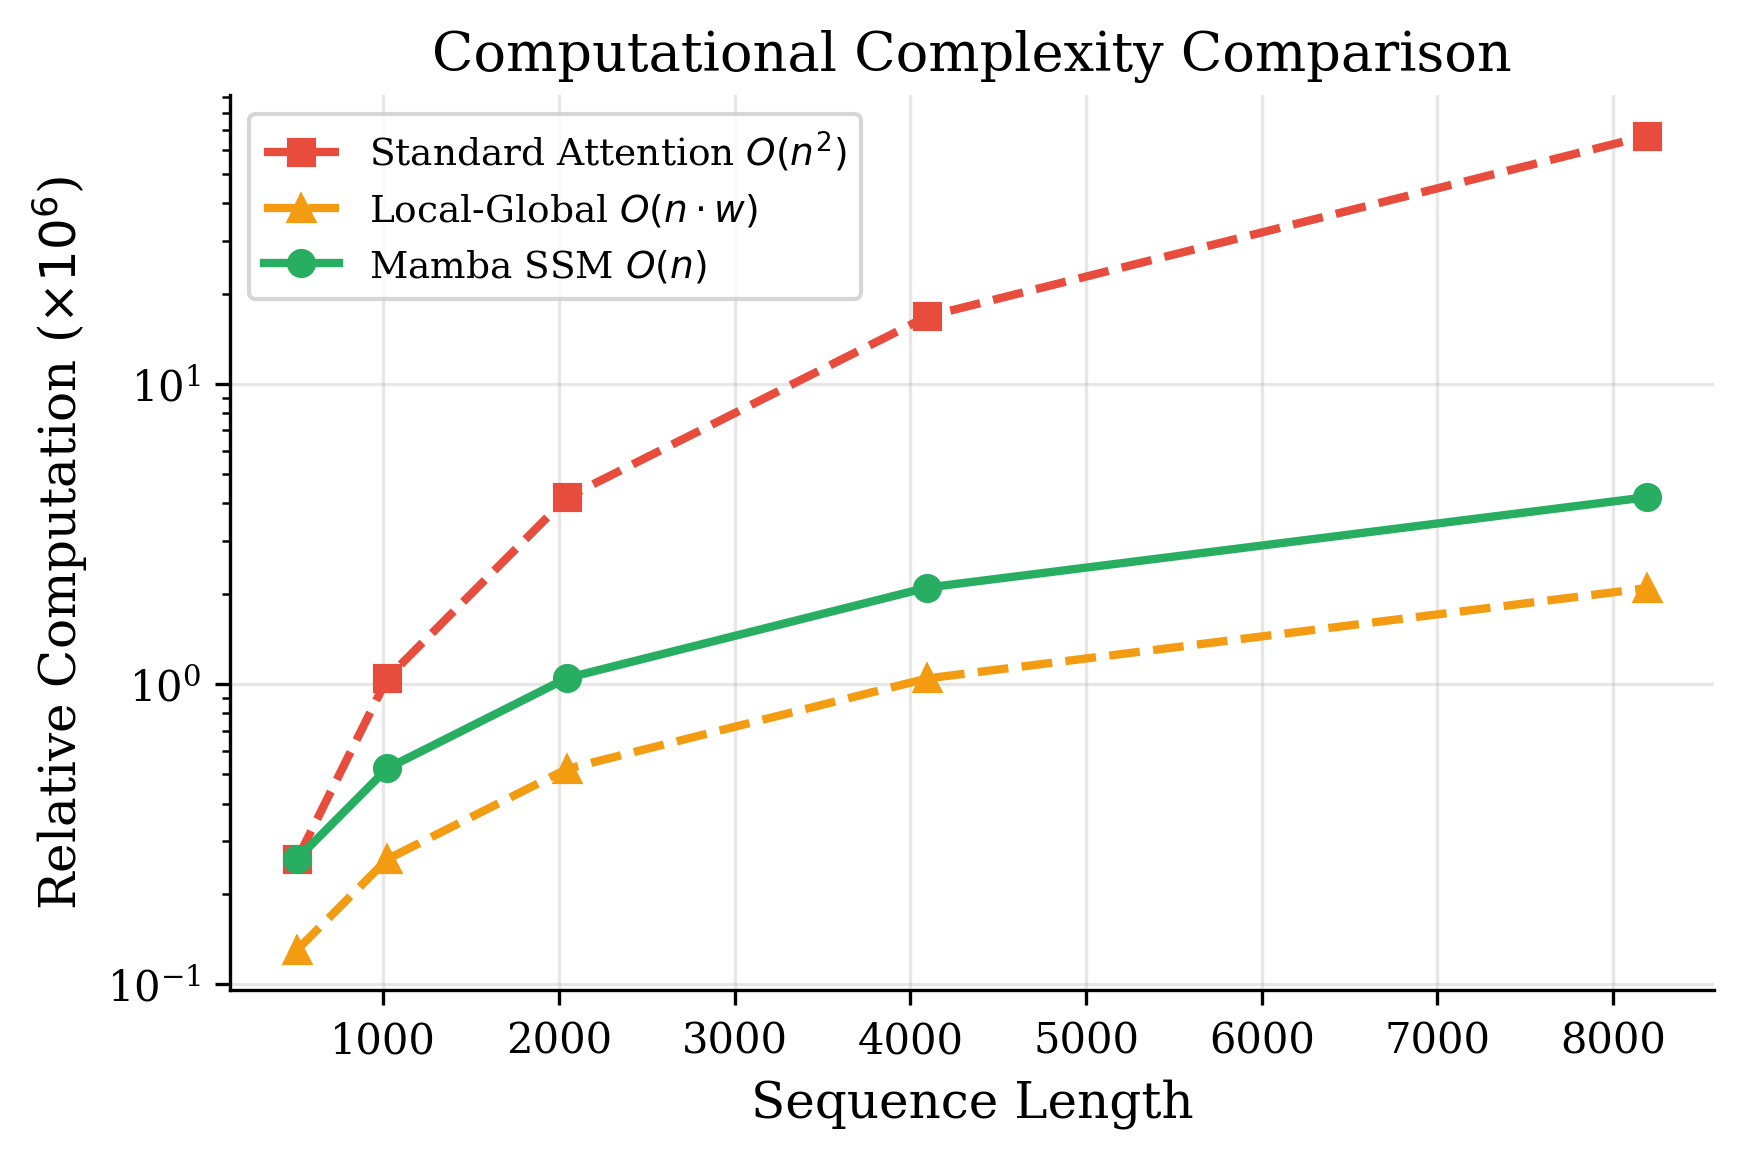
\includegraphics[width=\textwidth]{figures/complexity_comparison.png}
    \end{column}
  \end{columns}

  \vspace{0.2cm}
  {\small While Mamba V2 has 79.4M parameters, the Mamba SSM encoder operates in $O(n)$ linear complexity, making it significantly more efficient than standard $O(n^2)$ attention for long clinical documents.}
\end{frame}

\begin{frame}{Issue Resolution Timeline}
  \begin{center}
    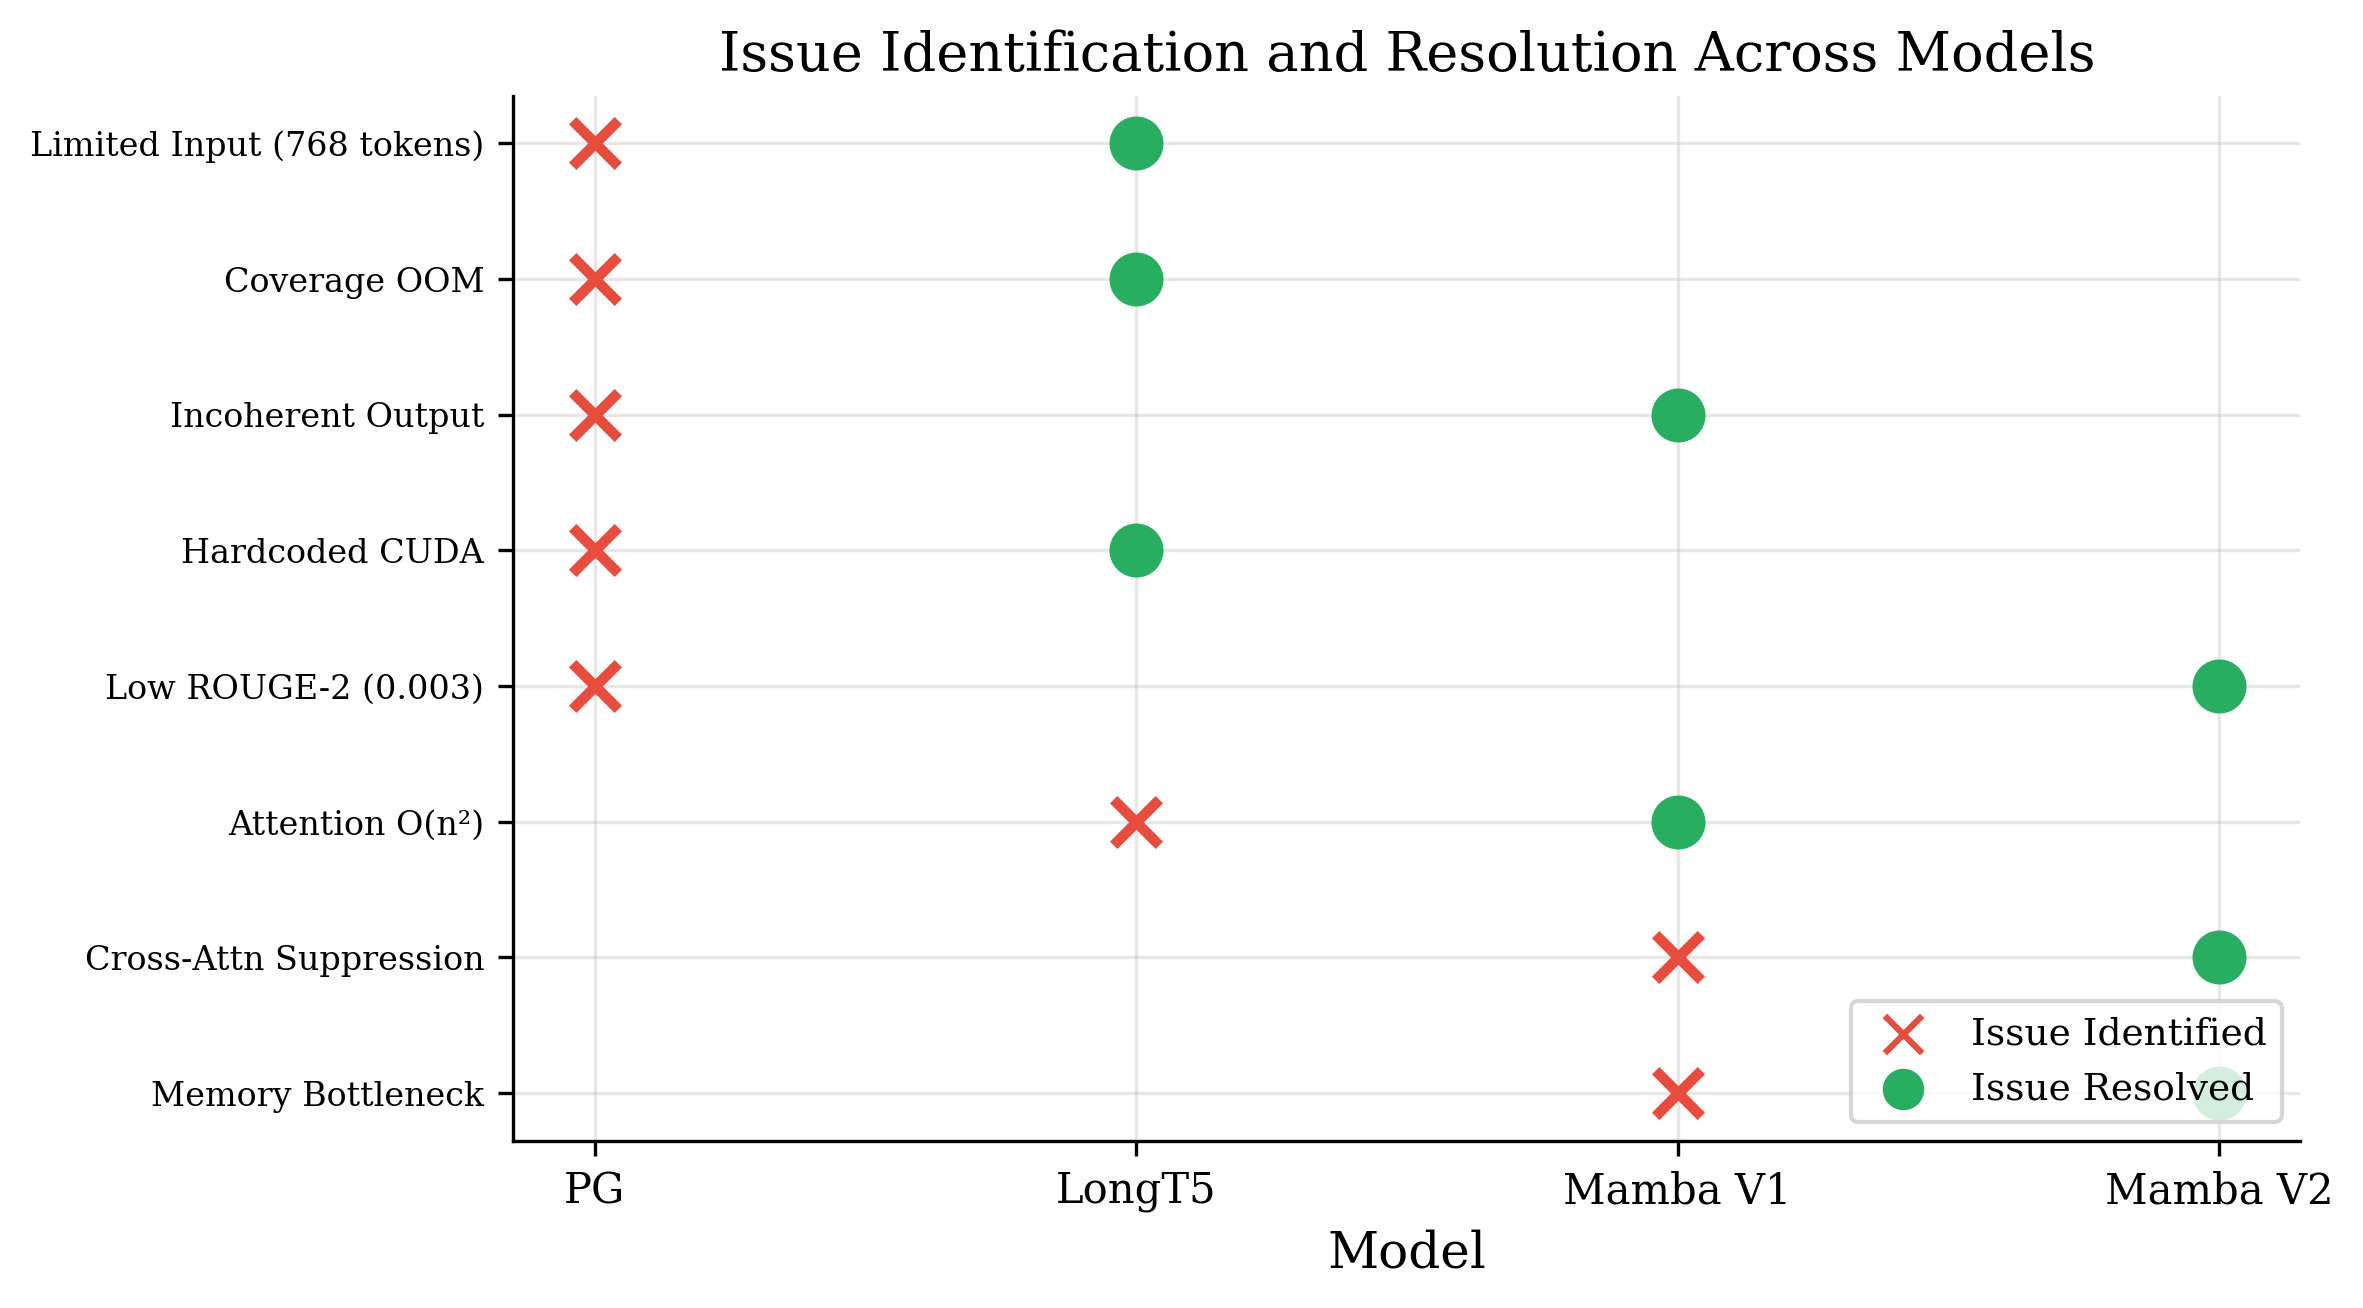
\includegraphics[width=0.7\textwidth]{figures/issue_resolution.png}
  \end{center}
  \vspace{-0.3cm}
  {\scriptsize Each successive model resolved its predecessor's limitations. Mamba V2 addresses all issues including cross-attention suppression and memory bottleneck.}
\end{frame}

\begin{frame}{Per-Sample Performance Analysis}
  \begin{columns}[T]
    \begin{column}{0.55\textwidth}
      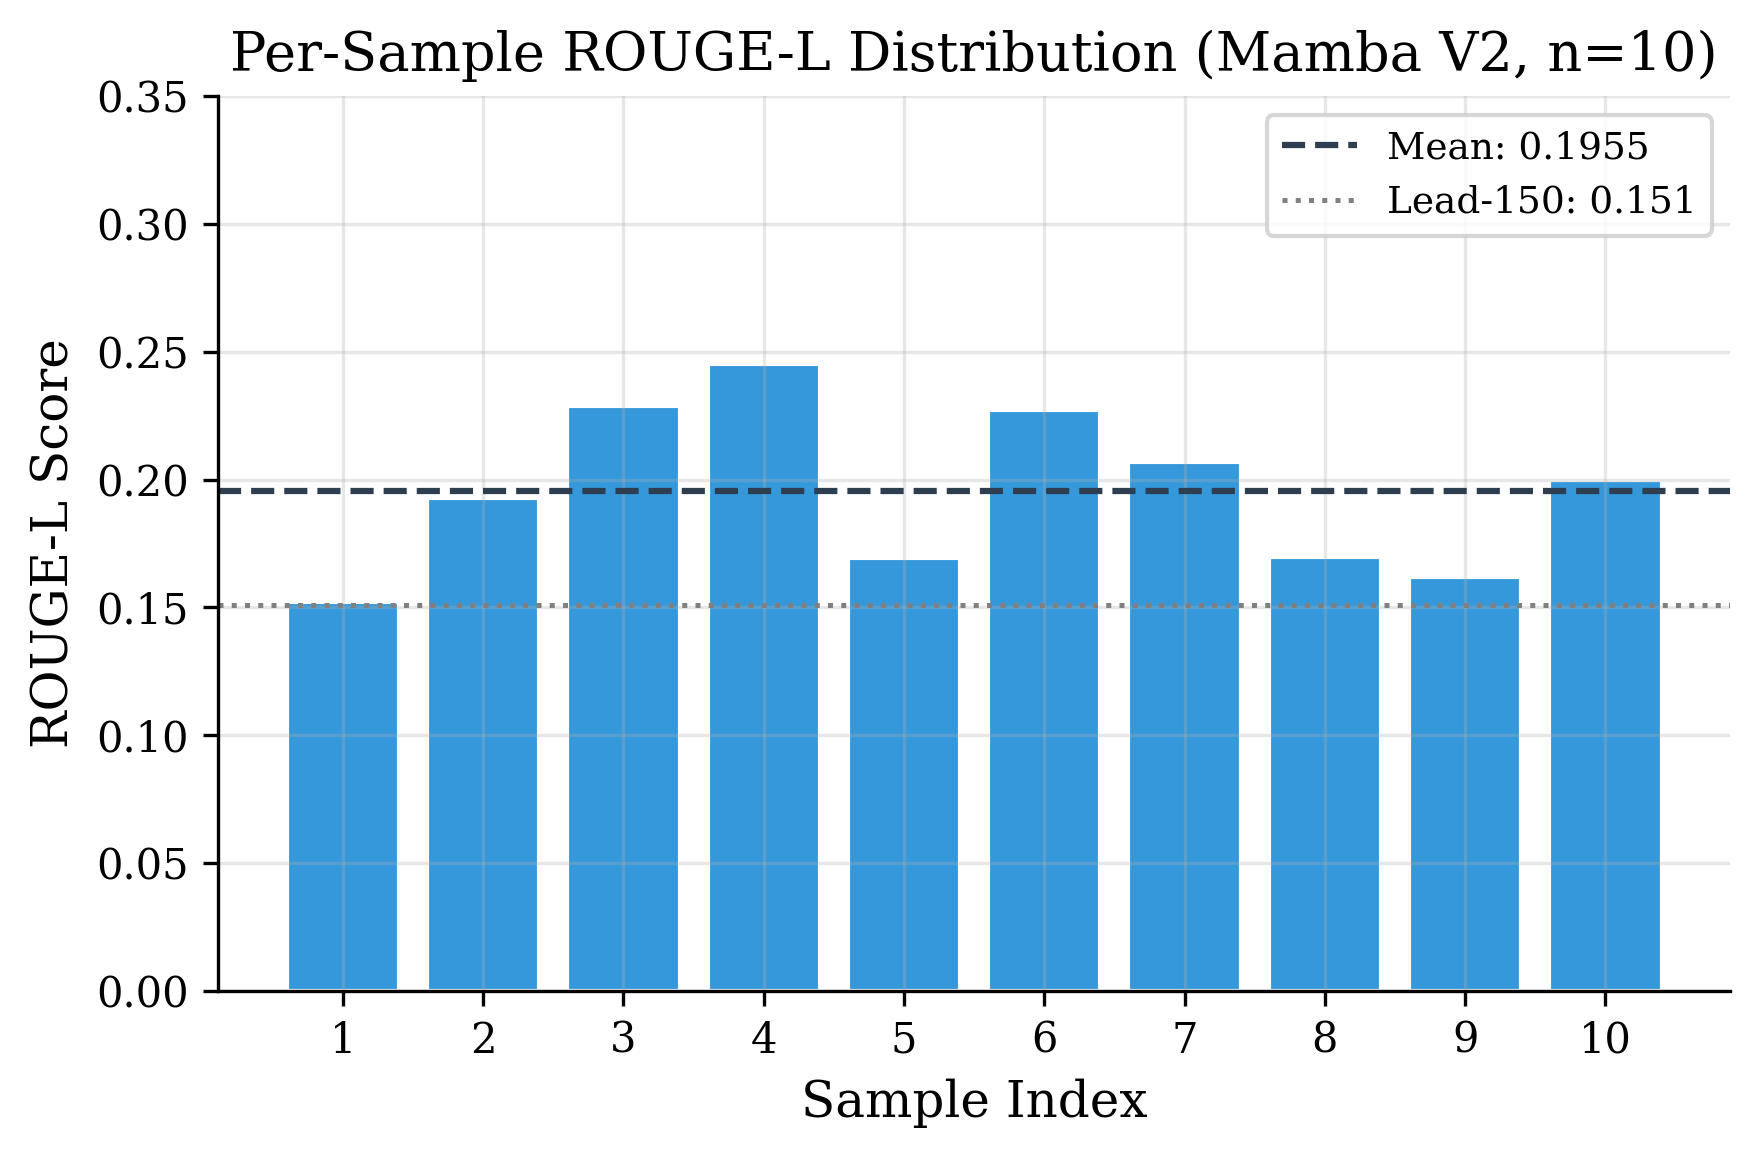
\includegraphics[width=\textwidth]{figures/sample_distribution.png}
    \end{column}
    \begin{column}{0.42\textwidth}
      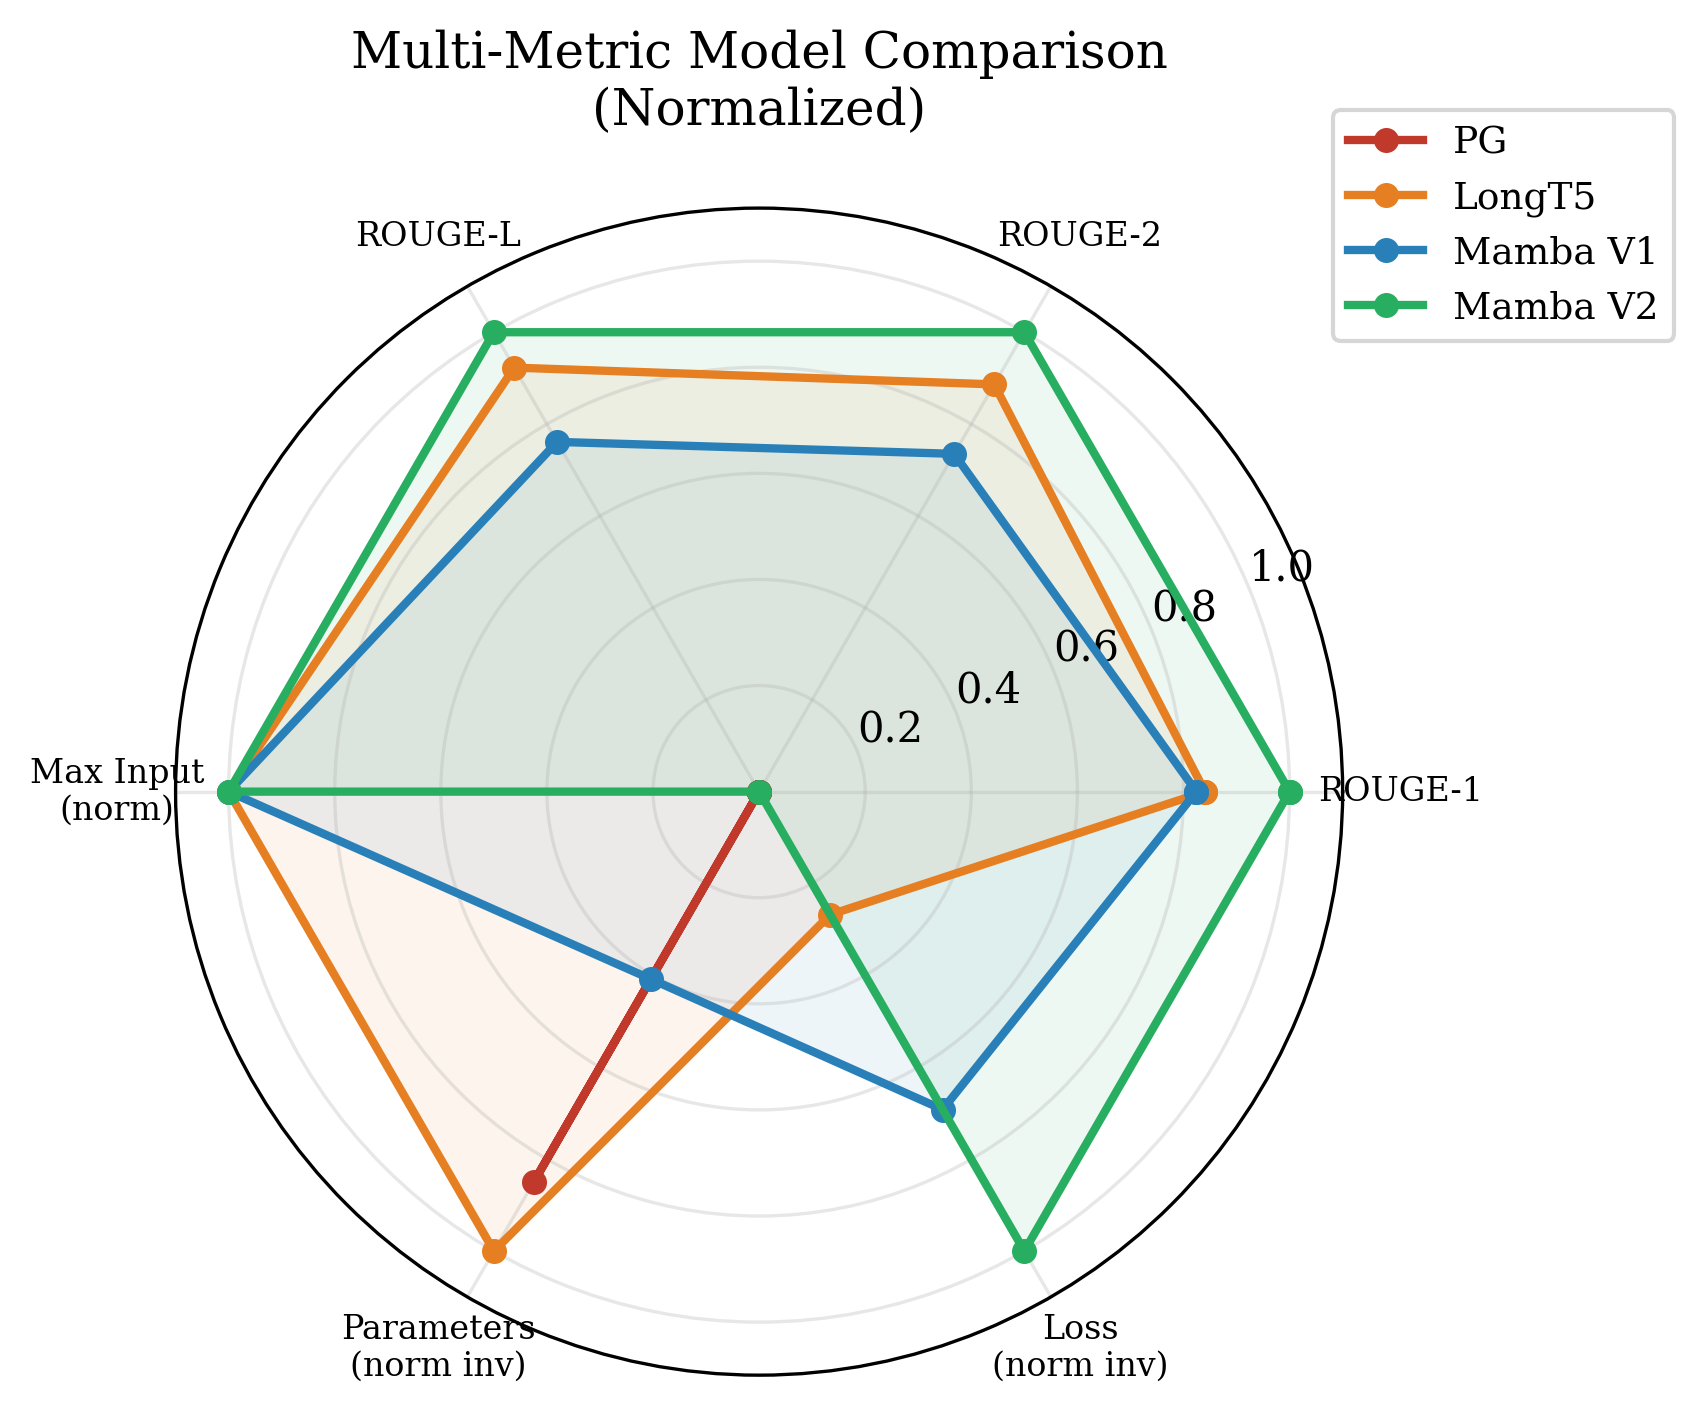
\includegraphics[width=\textwidth]{figures/radar_comparison.png}
    \end{column}
  \end{columns}

  \vspace{0.2cm}
  {\small Mamba V2 consistently outperforms the Lead-150 baseline across individual samples (left). The radar chart (right) shows Mamba V2 dominates across multiple evaluation dimensions.}
\end{frame}

\begin{frame}{Comprehensive Metrics Comparison}
  \begin{table}
    \centering
    \small
    \renewcommand{\arraystretch}{1.3}
    \begin{tabular}{l|cccc}
      \toprule
      \textbf{Metric} & \textbf{Pointer-Gen} & \textbf{LongT5} & \textbf{Mamba V1} & \textbf{Mamba V2} \\
      \midrule
      \rowcolor{lightgray} ROUGE-1 & 0.1814 & 0.3517 & 0.3484 & \textcolor{darkgreen}{\textbf{0.3840}} \\
      ROUGE-2 & 0.0030 & 0.1232 & 0.1027 & \textcolor{darkgreen}{\textbf{0.1386}} \\
      \rowcolor{lightgray} ROUGE-L & 0.0855 & 0.2185 & 0.1952 & \textcolor{darkgreen}{\textbf{0.2296}} \\
      \midrule
      Parameters & 22.5M & 12.5M & 52.1M & 79.4M \\
      \rowcolor{lightgray} Max Input (tokens) & 768 & 4,096 & 4,096 & 4,096 \\
      Max Target (tokens) & 192 & 256 & 512 & 512 \\
      \rowcolor{lightgray} Encoder Type & BiLSTM & Local-Global & BiMamba & BiMamba+ \\
      Attention Complexity & $O(n^2)$ & $O(n \cdot w)$ & $O(n)$ & $O(n)$ \\
      \rowcolor{lightgray} Copy Mechanism & \checkmark & $\times$ & $\times$ & \checkmark \\
      Final Loss & 4.80 & 4.20 & 3.25 & \textcolor{darkgreen}{\textbf{2.56}} \\
      \rowcolor{lightgray} Training Steps & 500 & --- & 40,000 & 150,000 (completed) \\
      \midrule
      \textbf{vs.\ Lead-150} & Below & Above & Above & \textcolor{darkgreen}{\textbf{+52.1\%}} \\
      \bottomrule
    \end{tabular}
  \end{table}
  \vspace{-0.1cm}
  {\small Mamba V2 achieves the best performance across all ROUGE metrics (best at step 130K) and the lowest validation loss (2.56 at 150K), validating the progressive architectural improvements. Training completed all 150,000 steps.}
\end{frame}

% ============================================================
% SECTION 7: EVALUATION BEYOND ROUGE
% ============================================================
\section{Clinical Evaluation Framework}

\begin{frame}{Limitations of ROUGE for Clinical Text}
  \small
  \begin{table}
    \centering
    \small
    \renewcommand{\arraystretch}{1.2}
    \begin{tabular}{lcc}
      \toprule
      \textbf{Problem} & \textbf{Example} & \textbf{ROUGE Verdict} \\
      \midrule
      Synonym blindness & ``HTN'' vs.\ ``hypertension'' & Different \\
      Negation insensitivity & ``has DM'' vs.\ ``denies DM'' & High overlap \\
      Number insensitivity & ``troponin 0.45'' vs.\ ``4.50'' & Nearly identical \\
      Multiple valid phrasings & Clinical synonymy & Penalizes variants \\
      Safety blindness & Hallucinated medications & High (similar terms) \\
      \bottomrule
    \end{tabular}
  \end{table}

  \vspace{0.1cm}

  \begin{block}{Proposed 4-Gate Clinical Evaluation Framework}
    \small
    \begin{enumerate}\setlength{\itemsep}{0pt}
      \item \textbf{Gate 1 -- Safety:} PHI leakage (0\%), negation consistency ($<$2\%), contradiction rate ($<$15\%)
      \item \textbf{Gate 2 -- Clinical Accuracy:} MEDCON (UMLS F1), Medical Entity F1, ICD-10 coverage
      \item \textbf{Gate 3 -- Semantic Quality:} BERTScore (Bio\_ClinicalBERT), BARTScore
      \item \textbf{Gate 4 -- Surface Overlap:} ROUGE-1/2/L, Repetition rate, Length ratio
    \end{enumerate}
  \end{block}
\end{frame}

\begin{frame}{Clinical Metrics: Mathematical Definitions}
  \small
  \begin{columns}[T]
    \begin{column}{0.48\textwidth}
      \textbf{BERTScore} (Semantic Similarity):
      \vspace{-0.15cm}
      \begin{align}
        P &= \frac{1}{|\hat{y}|}\sum_j \max_i \cos(h_j, h_i) \nonumber \\
        R &= \frac{1}{|y|}\sum_i \max_j \cos(h_i, h_j) \nonumber \\
        F_1 &= \frac{2PR}{P+R} \nonumber
      \end{align}
      \vspace{-0.3cm}
      {\scriptsize Using Bio\_ClinicalBERT embeddings.}

      \vspace{0.1cm}
      \textbf{MEDCON} (UMLS Concept F1):
      \vspace{-0.1cm}
      \begin{equation}
        F_1 = \frac{2 \cdot |\text{CUI}_{\text{pred}} \cap \text{CUI}_{\text{ref}}|}{|\text{CUI}_{\text{pred}}| + |\text{CUI}_{\text{ref}}|} \nonumber
      \end{equation}
    \end{column}
    \begin{column}{0.48\textwidth}
      \textbf{SummaC} (Factual Consistency):
      \begin{enumerate}\setlength{\itemsep}{0pt}
        \item Split summary into sentences
        \item NLI against source: entail / contradict / neutral
        \item Aggregate consistency score
      \end{enumerate}

      \vspace{0.1cm}
      \textbf{Negation Consistency:}
      \vspace{-0.1cm}
      \begin{equation}
        \text{Error} = \frac{|\text{flipped negations}|}{|\text{total negations}|} \nonumber
      \end{equation}
      \vspace{-0.2cm}
      {\scriptsize Detects ``denies X'' $\rightarrow$ ``has X'' flips.}

      \vspace{0.1cm}
      \textbf{Length Ratio:}
      \vspace{-0.1cm}
      \begin{equation}
        r = \frac{|\text{generated}|}{|\text{reference}|} \nonumber
      \end{equation}
      \vspace{-0.2cm}
      {\scriptsize Target: $r \approx 1.0$ for balanced summaries.}
    \end{column}
  \end{columns}
\end{frame}

% ============================================================
% SECTION 8: CONCLUSION
% ============================================================
\section{Conclusion}

\begin{frame}{Conclusion}
  \begin{block}{Summary}
    \small We presented a systematic progression through four architectures for clinical data summarization, each addressing specific limitations of its predecessor.
  \end{block}

  \vspace{0.1cm}
  \small
  \begin{columns}[T]
    \begin{column}{0.48\textwidth}
      \textbf{Key Findings:}
      \begin{enumerate}\setlength{\itemsep}{0pt}
        \item \textbf{PG}: Baseline; limited by 768 tokens \& OOM
        \item \textbf{LongT5}: 4,096 tokens via local-global attention
        \item \textbf{Mamba V1}: Linear SSM encoding + memory compression
        \item \textbf{Mamba V2}: Gate fix + bypass + SwiGLU $\rightarrow$ \textbf{best}
      \end{enumerate}
    \end{column}
    \begin{column}{0.48\textwidth}
      \textbf{Final Results (Mamba V2):}
      \begin{itemize}\setlength{\itemsep}{0pt}
        \item R-1: \textbf{0.3840} (+111.7\% vs.\ PG)
        \item R-2: \textbf{0.1386} (+4,520\% vs.\ PG)
        \item R-L: \textbf{0.2296} (+168.5\% vs.\ PG)
        \item 150K steps completed; val loss \textbf{2.56}
        \item \textbf{Surpasses Lead-150} across all metrics
      \end{itemize}

      \vspace{0.1cm}
      \textbf{Future Work:}
      \begin{itemize}\setlength{\itemsep}{0pt}
        \item Copy mechanism for exact term copying
        \item Clinical eval metrics (MEDCON, BERTScore)
        \item Domain-specific pre-training
        \item Larger Mamba configurations
      \end{itemize}
    \end{column}
  \end{columns}
\end{frame}

\begin{frame}{Acknowledgments \& References}
  \textbf{Acknowledgments:}\\
  We thank the MIMIC-IV team at PhysioNet for providing the clinical dataset, and our course instructor for guidance throughout this project.

  \vspace{0.4cm}

  \textbf{Key References:}
  \begin{enumerate}
    \item[\tiny{[1]}] {\scriptsize See, A., Liu, P. J., \& Manning, C. D. (2017). Get To The Point: Summarization with Pointer-Generator Networks. \textit{ACL 2017}.}
    \item[\tiny{[2]}] {\scriptsize Guo, M., et al. (2022). LongT5: Efficient Text-To-Text Transformer for Long Sequences. \textit{NAACL 2022}.}
    \item[\tiny{[3]}] {\scriptsize Gu, A., \& Dao, T. (2023). Mamba: Linear-Time Sequence Modeling with Selective State Spaces. \textit{arXiv:2312.00752}.}
    \item[\tiny{[4]}] {\scriptsize Johnson, A., et al. (2023). MIMIC-IV: A freely accessible electronic health record dataset. \textit{Scientific Data}.}
    \item[\tiny{[5]}] {\scriptsize Vaswani, A., et al. (2017). Attention Is All You Need. \textit{NeurIPS 2017}.}
    \item[\tiny{[6]}] {\scriptsize Shazeer, N. (2020). GLU Variants Improve Transformer. \textit{arXiv:2002.05202}.}
    \item[\tiny{[7]}] {\scriptsize Zhang, B., \& Sennrich, R. (2019). Root Mean Square Layer Normalization. \textit{NeurIPS 2019}.}
  \end{enumerate}
\end{frame}

% ============================================================
% THANK YOU
% ============================================================
{
\setbeamertemplate{footline}{}
\begin{frame}
  \begin{center}
    \vspace{1.5cm}
    {\Huge \textcolor{ieeeblue}{Thank You}}\\
    \vspace{0.8cm}
    {\Large Questions?}\\
    \vspace{1.0cm}
    {\normalsize
      AIE315: Natural Language Processing\\
      S6 AIE Batch B -- Group 5\\
      \vspace{0.3cm}
      \textit{Clinical Data Summarization}\\
      \textit{A Comparative Study of Pointer-Generator, LongT5, and Mamba-Transformer Hybrid Models}
    }
  \end{center}
\end{frame}
}

\end{document}
